%%%%%%%%%%%%%%%%%%%%%%%%%%%%%%%%%%%%%%%%%%%%%%%%%%%%%%%%%%%%%%%%%%%%%%%%%%%%%%%%%%%%%
\section{Introduction}\label{sec:mtd_intro}
%%%%%%%%%%%%%%%%%%%%%%%%%%%%%%%%%%%%%%%%%%%%%%%%%%%%%%%%%%%%%%%%%%%%%%%%%%%%%%%%%%%%%

HAWC's current software suite, plugins to 3ML, does not fully utilize computational advancements of recent decades.
Said advancements include the proliferation of Graphical Processing Units (GPUs), and multithreading on multi-core processors.
The analysis described in \Cref{sec:glory_duck} took up to 3 months of human time waiting for the full gambit of data analysis and simulation of background to run.
Additionaly, with the addition of a 2D binning scheme, $f_\mathrm{hit}$ and NN, the compute time is expected to grow.
Although excessive computing time was, in part, from an intense use of a shared computing cluster, it was evident that there was room for improvement.
In HAWC's next generation dSph DM search, I decided to develop codes that would utilize the multi-core processors on modern high performance computing clusters.
The results of this work are featured in this chapter and brought a human timing improvement to computation that scales as $1/N$ where $N$ is the number of threads.

%%%%%%%%%%%%%%%%%%%%%%%%%%%%%%%%%%%%%%%%%%%%%%%%%%%%%%%%%%%%%%%%%%%%%%%%%%%%%%%%%%%%%
\section{Dataset and Background}\label{sec:mtd_databgd}
%%%%%%%%%%%%%%%%%%%%%%%%%%%%%%%%%%%%%%%%%%%%%%%%%%%%%%%%%%%%%%%%%%%%%%%%%%%%%%%%%%%%%

This section enumerates the data and background methods used for HAWC's multi-threaded study of dSphs.
\Cref{sec:mtd_data} and \Cref{sec:mtd_tools} are most useful for fellow HAWC collaborators looking to replicate a multithreaded dSph DM search.

%%%%%%%%%%%%%%%%%%%%%%%%%%%%%%%%%%%%%%%%%%%%%%%
\subsection{Itemized HAWC files}\label{sec:mtd_data}
%%%%%%%%%%%%%%%%%%%%%%%%%%%%%%%%%%%%%%%%%%%%%%%

\begin{itemize}
    \item Detector Resolution: \texttt{refit-Pass5-Final-NN-detRes-zenith-dependent.root}
    \item Data Map: \texttt{Pass5-Final-NN-maptree-ch103-ch1349-zenith-dependent.root}
    \item Spectral Dictionary: \texttt{HDMSpectra\_dict\_gamma.npy}
\end{itemize}

% %%%%%%%%%%%%%%%%%%%%%%%%%%%%%%%%%%%%%%%%%%%%%%%
\subsection{Software Tools and Development}\label{sec:mtd_tools}
%%%%%%%%%%%%%%%%%%%%%%%%%%%%%%%%%%%%%%%%%%%%%%%

This analysis was performed using HAL and 3ML \cite{Abeysekara_2017, vianello2015multimission} in Python version 3.
I built software in collaboration with Michael Martin and Letrell Harris to implement the \emph{Dark Matter Spectra from the Electroweak to the Planck Scale} (HDM) \cite{HDMSpectra} and dSphs spatial model from \cite{DM_Strigari20} for HAWC analysis.
A NumPy dictionary of HDM was made for Py3.
The corresponding Python3 file is \texttt{HDMSpectra\_dict\_gamma.npy}.
These files can also be used for decay channels and tools are provided in HDM's \href{https://github.com/nickrodd/HDMSpectra/tree/master}{git repository} \cite{HDMSpectra}.
The analysis was performed using the Neural Network energy estimator for Pass 5.F.
A description of this estimator was provided in \Cref{sec:hawc}.\todo{define a subsection when it's written}
All other software used for data analysis, DM profile generation, and job submission to SLURM are also kept in my sandbox in the \href{https://gitlab.com/hawc-observatory/sandboxes/salaza82/dark_matter_hawc}{Dark Matter HAWC} project.
The above repository also incorporates the model inputs used previously in Glory Duck, described in \Cref{sec:glory_duck}

%%%%%%%%%%%%%%%%%%%%%%%%%%%%%%%%%%%%%%%%%%%%%%%
\subsection{Data Set and Background Description} \label{sec:mtd_data_bkgd}
%%%%%%%%%%%%%%%%%%%%%%%%%%%%%%%%%%%%%%%%%%%%%%%

The HAWC data maps used for this analysis contain 2565 days of data between runs 2104 (\todo{Day start}) and 7476 (\todo{day end}).
They were generated from pass 4.0 reconstruction.
The analysis is performed using the NN energy estimator with bin list:

\begin{itemize}
    \item[] \texttt{B1C0Ea}, \texttt{B1C0Eb}, \texttt{B1C0Ec}, \texttt{B1C0Ed}, \texttt{B1C0Ee}, \texttt{B2C0Ea}, \texttt{B2C0Eb}, \texttt{B2C0Ec}, \texttt{B2C0Ed}, \texttt{B2C0Ee}, \texttt{B3C0Ea}, \texttt{B3C0Eb}, \texttt{B3C0Ec}, \texttt{B3C0Ed}, \texttt{B3C0Ee}, \texttt{B3C0Ef}, \texttt{B4C0Eb}, \texttt{B4C0Ec}, \texttt{B4C0Ed}, \texttt{B4C0Ee}, \texttt{B4C0Ef}, \texttt{B5C0Ec}, \texttt{B5C0Ed}, \texttt{B5C0Ee}, \texttt{B5C0Ef}, \texttt{B5C0Eg}, \texttt{B6C0Ed}, \texttt{B6C0Ee}, \texttt{B6C0Ef}, \texttt{B6C0Eg}, \texttt{B6C0Eh}, \texttt{B7C0Ee}, \texttt{B7C0Ef}, \texttt{B7C0Eg}, \texttt{B7C0Eh}, \texttt{B7C0Ei}, \texttt{B8C0Ee}, \texttt{B8C0Ef}, \texttt{B8C0Eg}, \texttt{B8C0Eh}, \texttt{B8C0Ei}, \texttt{B8C0Ej}, \texttt{B9C0Ef}, \texttt{B9C0Eg}, \texttt{B9C0Eh}, \texttt{B9C0Ei}, \texttt{B9C0Ej}, \texttt{B10C0Eg}, \texttt{B10C0Eh}, \texttt{B10C0Ei}, \texttt{B10C0Ej}, \texttt{B10C0Ek}, \texttt{B10C0El}
\end{itemize}
Bin 0 was excluded as it has substantial hadronic contamination and poor angular resolution.

Background considerations and source selection was identical to \Cref{sec:gd_databgd}, and no additional arguements are provided here.
Many of the HAWC systematics explored in \Cref{sec:hawc_systematic} also apply for this DM search and are not added upon here.

%%%%%%%%%%%%%%%%%%%%%%%%%%%%%%%%%%%%%%%%%%%%%%%%%%%%%%%%%%%%%%%%%%%%%%%%%%%%%%%%%%%%%
\section{Analysis}\label{sec:mtd_analysis}
%%%%%%%%%%%%%%%%%%%%%%%%%%%%%%%%%%%%%%%%%%%%%%%%%%%%%%%%%%%%%%%%%%%%%%%%%%%%%%%%%%%%%

The analysis and its systematics are almost identical to \Cref{sec:gd_analysis}.
Importantly, we use the same \Cref{eq:id_dm_flux} and \Cref{eq:jfactor} for estimating the gamma-ray flux at HAWC from our sources.
We add on to the previous study with a search for DM decay.
The flux equations for DM decay are
\iddmdecay[\gamma]

with a new quantity, the \D factor, defined as
\dfactor
Software was written to accomodate DM decay from dSphs, however decay profiles were not received from \LS by the time of writing this tehsis.

%%%%%%%%%%%%%%%%%%%%%%%%%%%%%%%%%%%%%%%%%%%%%%%%%%
\subsection{$\frac{dN_\gamma}{dE_\gamma}$ - Particle Physics Component}\label{sec:mtd_particlephysics}
%%%%%%%%%%%%%%%%%%%%%%%%%%%%%%%%%%%%%%%%%%%%%%%%%%

For these spectra, we import HDM with Electroweak (EW) corrections and additional corrections for neutrinos above the EW scale \cite{HDMSpectra}.
The spectrum is implemented as a model script in astromodels for 3ML.
A comprehensive description of EW corrections and neutrino considerations are provided later in \todo{refeance MM nu duck}.

\begin{figure}[t]
    \centering{
        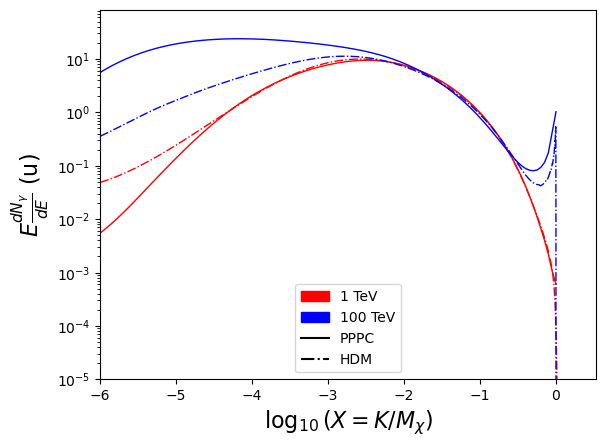
\includegraphics[scale=0.8]{figures/mtd_hawc_dm/pppc_vs_hdm.png}
    }
    \caption{Difference between spectral hypotheses from PPPC \cite{Cirelli_2011} and HDM \cite{HDMSpectra}. Shown is the expected DM annihilation spectrum for $\chi\chi \rightarrow W^-W^+$. Solid lines are spectral models with EW corrections from the PPPC. Dash-dot lines are spectral models from HDM. Red lines are models for $M_\chi = 1$ TeV. Blue lines represent models for $M_\chi = 100$ TeV.}
    \label{fig:pppc_vs_hdm}
\end{figure}

\Cref{fig:pppc_vs_hdm} demonstrates the impact of changes from HDM on DM
annihilation to W bosons.
A class in astromodels was developed to include HDM and is aptly named \texttt{HDMSpectra} within \texttt{DM\_models.py}.
The SM DM annihilation channels studied here are $\chi\chi \rightarrow$:
\begin{itemize}
    \item[] $e^+e^-$, $\mu^+\mu^-$, $\tau^+\tau^-$,$b\bar{b}$, $t\bar{t}$, $gg$, $W^+W^-$, $ZZ$, $c\bar{c}$, $u\bar{u}$, $d\bar{d}$, $s\bar{s}$, $\nu_e \overline{\nu_e}$, $\nu_\mu \overline{\nu_\mu}$, $\nu_\tau \overline{\nu_\tau}$, $\gamma\gamma$, $hh$.
\end{itemize}
For $\gamma\gamma$ and $ZZ$, a substantial fraction of the signal photons are expected to have total energy equal $m_\chi$ \cite{HDMSpectra}.
This introduces a $\delta$-function that is much narrower than the energy resolution of the HAWC detector.
To ensure that this feature is not lost in the likelihood fits, the 'line' feature is convolved with a gausian kernel with a $1\sigma$ width of $0.05 \cdot m_\chi$ and total kernel window of $\pm4\sigma$.
This difers from HAWC's previous line study where 30\% of HAWC's energy resolution was used for the kernel \cite{HAWC_dm_gammalines}.
The NN energy estimator's strength compared to $f_\mathrm{hit}$ at low gamma-ray energy enables smaller resolutions in addition to low energy tails in the spectral models \cite{HDMSpectra}.
$\chi\chi \rightarrow \gamma\gamma$ and $ZZ$ spectral hypotheses are shown in \Cref{fig:hdm_gamma_lines}.
Spectral models for the remaining annihilation channels are plotted for each $m_\chi$ in \Cref{fig:apdx_mtd_spectra}.

\begin{figure}[t]
    \centering{
    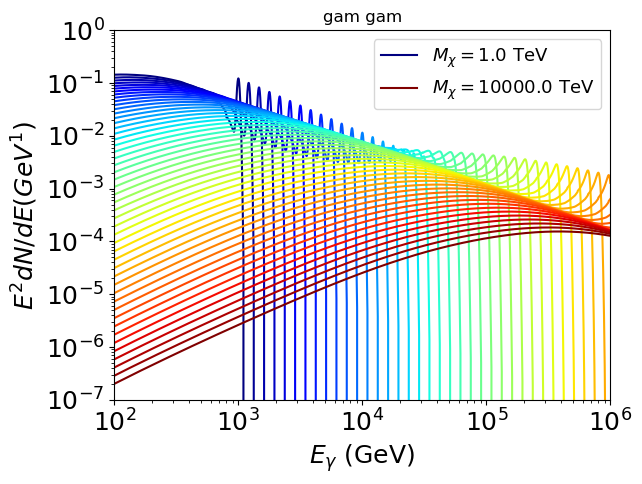
\includegraphics[scale=0.5]{figures/mtd_hawc_dm/hdm_gammagamma.png}
    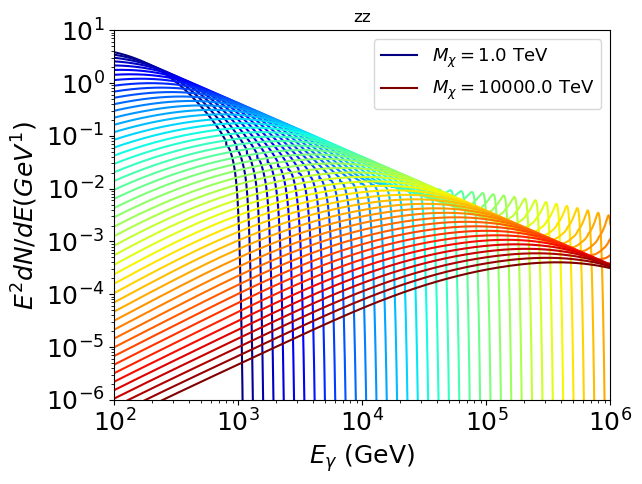
\includegraphics[scale=0.5]{figures/mtd_hawc_dm/hdm_zz.png}
    }
    \caption{Photon spectra for $\chi\chi \rightarrow \gamma\gamma$ (left) and $\chi\chi \rightarrow ZZ$ (right) after gaussian convolution of line features. Both spectra have $\delta$-features at photon energies equal to the DM mass. Bluer lines are annihilation spectra with lower DM mass. Redder lines are spectra from larger DM mass. All Spectral models are sourced from the Heavy Dark Matter models \cite{HDMSpectra}. Axes are drawn roughly according to the energy sensitivity of HAWC.}
    \label{fig:hdm_gamma_lines}
\end{figure}

%%%%%%%%%%%%%%%%%%%%%%%%%%%%%%%%%%%%%%%%%%%%%%%%%%
\subsection{\J and \D - Astrophysical Components}\label{sec:mtd_spatialmodel}
%%%%%%%%%%%%%%%%%%%%%%%%%%%%%%%%%%%%%%%%%%%%%%%%%%

The J-factor profiles for each source are imported from Louis Strigari et al. (referred to with \LS) \cite{DM_Strigari20}.
Profiles in $\frac{d\J}{d\Omega} (\theta)$ up to $\theta = 0.5^{\circ}$ were provided directly from the authors.
Map generation from these profiles were almost identical to \Cref{sec:gd_spatialmodel} except that a higher order trapezoidal integral was used for the normalization of the square, uniformly-spaced map:
\TrapIntegral
$\mathcal{K}$ is either \J or \D for the spatial distributions of annihilation or decay respectively.
$p$ is the angular side of one pixel in the map.
$w_{i,j}$ is a weight assigned the following ways:
\begin{itemize}
    \item[] $w_{i,j} = 1$ if $(\theta_{i,j}, \phi_{i,j})$ is fully within the region of integration
    \item[] $w_{i,j} = 1/2$ if $(\theta_{i,j}, \phi_{i,j})$ is on an edge of the region of integration
    \item[] $w_{i,j} = 1/4$ if $(\theta_{i,j}, \phi_{i,j})$ is on a corner of the region of integration
\end{itemize}
\Cref{fig:ls20_jfac_maps} shows the median and $\pm1\sigma$ maps used as input for DM annihilation studied by \LS.

\begin{figure}[t]
    \centering{
    \begin{tabular}{cccc}
        Source & $-1 \sigma$ & Mean & $+1 \sigma$ \\
        \rotatebox[origin=c]{90}{Coma Berenices} &
        \raisebox{-.5\height}{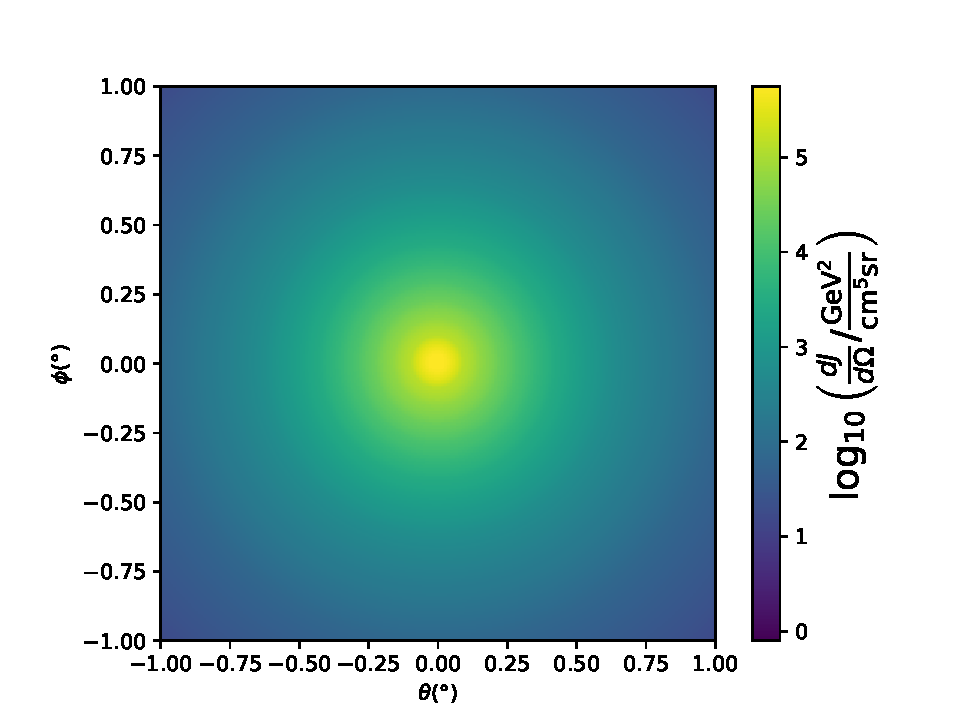
\includegraphics[scale=0.275]{figures/mtd_hawc_dm/ComaBerenices_Jm1_plot.pdf}} &
        \raisebox{-.5\height}{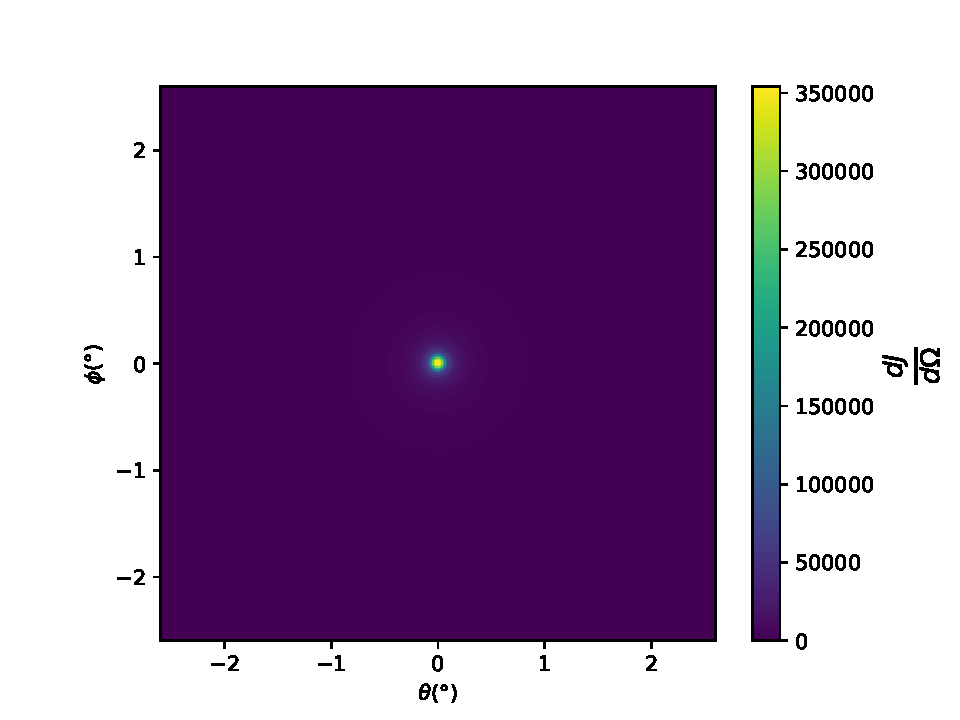
\includegraphics[scale=0.275]{figures/mtd_hawc_dm/ComaBerenices_J_plot.pdf}} &
        \raisebox{-.5\height}{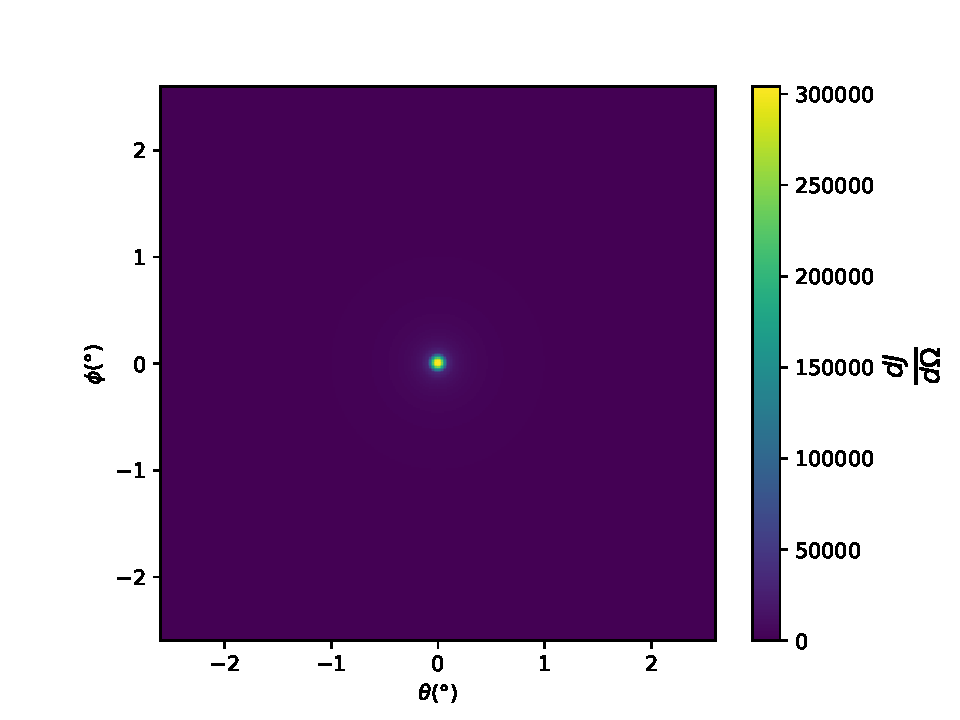
\includegraphics[scale=0.275]{figures/mtd_hawc_dm/ComaBerenices_Jp1_plot.pdf} }\\
        \rotatebox[origin=c]{90}{Draco} &
        \raisebox{-.5\height}{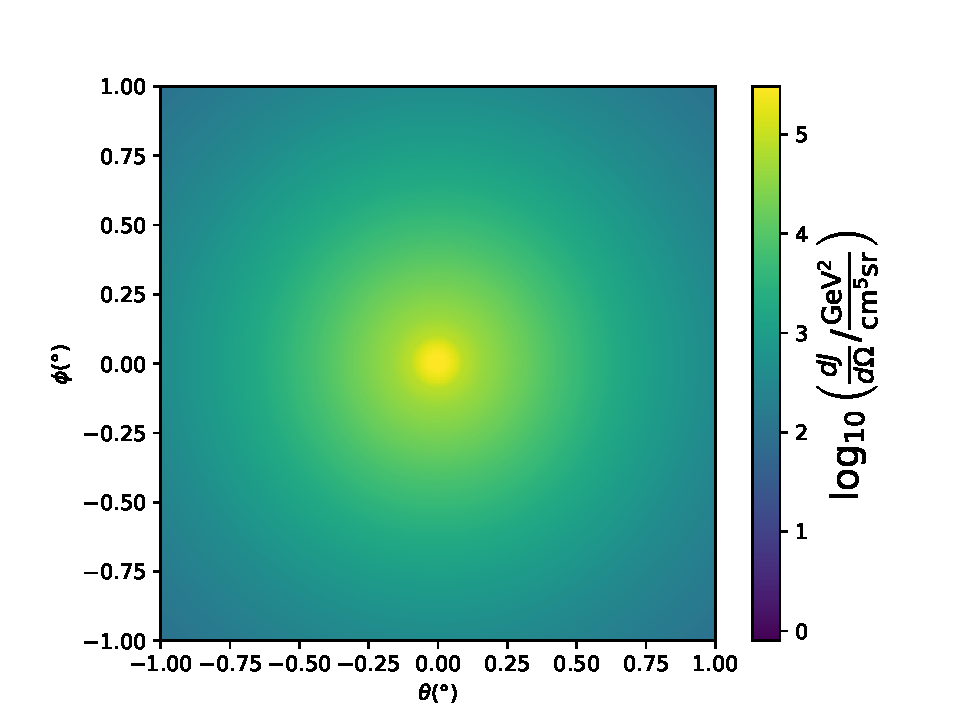
\includegraphics[scale=0.275]{figures/mtd_hawc_dm/Draco_Jm1_plot.pdf}} &
        \raisebox{-.5\height}{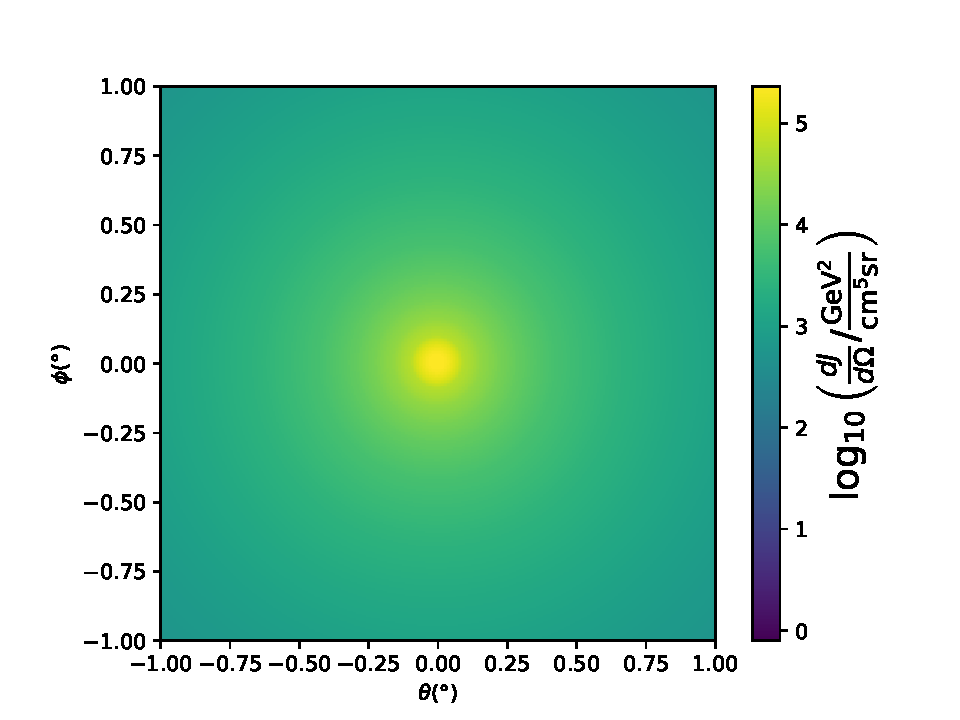
\includegraphics[scale=0.275]{figures/mtd_hawc_dm/Draco_J_plot.pdf}} &
        \raisebox{-.5\height}{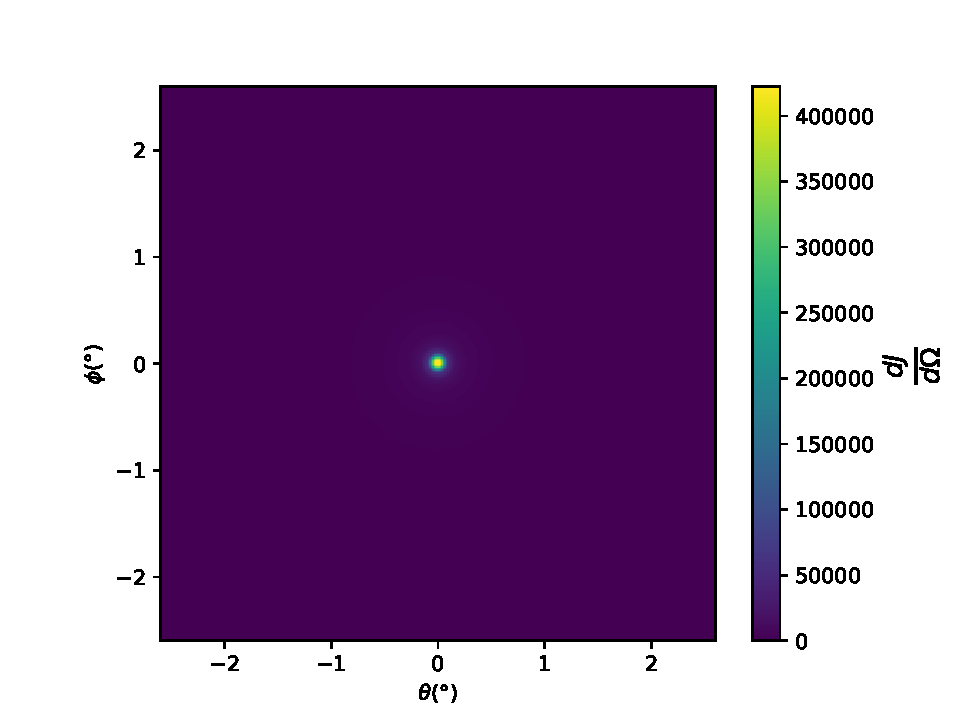
\includegraphics[scale=0.275]{figures/mtd_hawc_dm/Draco_Jp1_plot.pdf}} \\
        \rotatebox[origin=c]{90}{Segue1} &
        \raisebox{-.5\height}{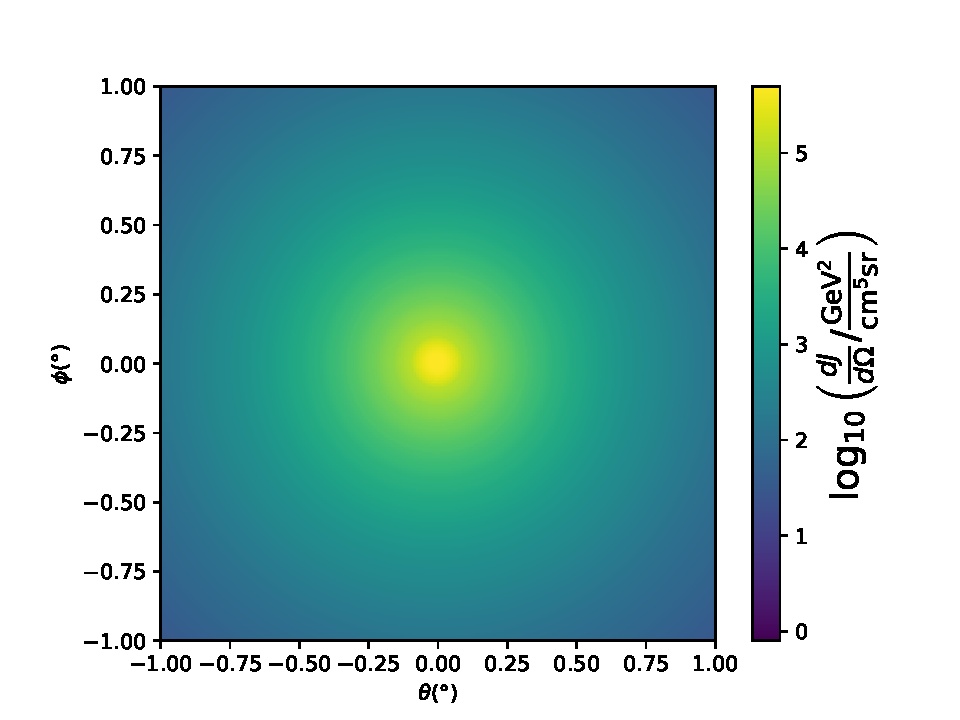
\includegraphics[scale=0.275]{figures/mtd_hawc_dm/Segue1_Jm1_plot.pdf}} &
        \raisebox{-.5\height}{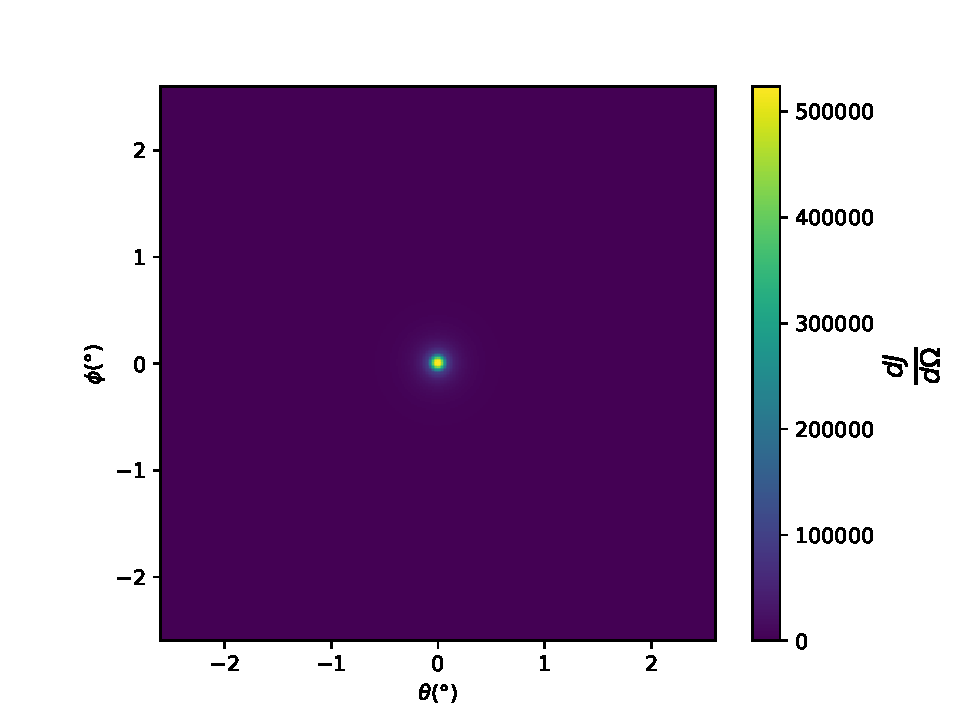
\includegraphics[scale=0.275]{figures/mtd_hawc_dm/Segue1_J_plot.pdf}} &
        \raisebox{-.5\height}{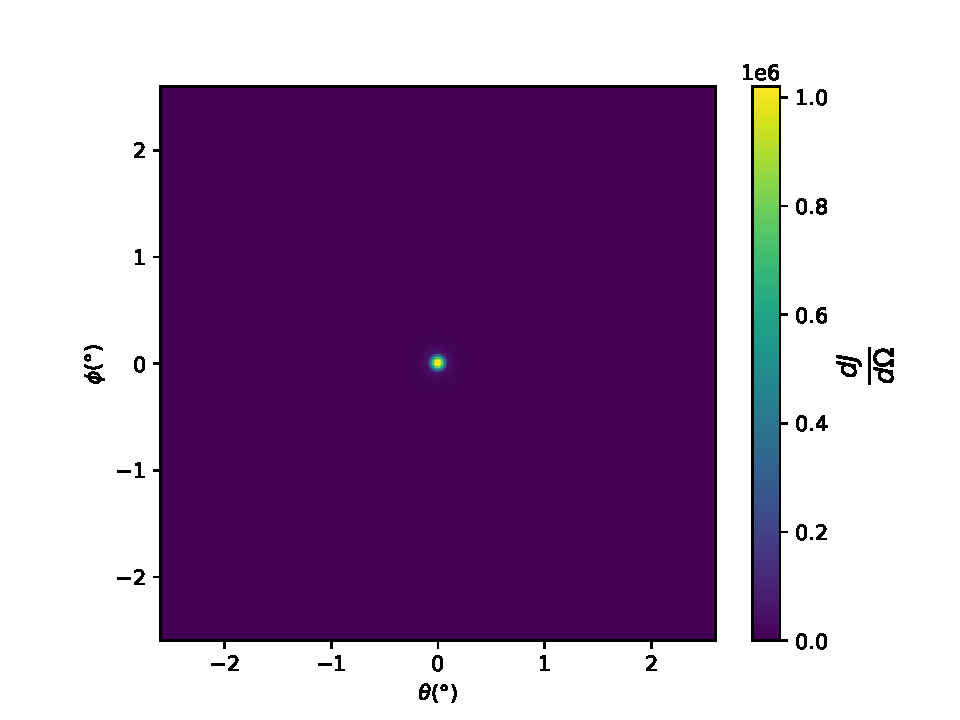
\includegraphics[scale=0.275]{figures/mtd_hawc_dm/Segue1_Jp1_plot.pdf}} \\
        \rotatebox[origin=c]{90}{Sextans} &
        \raisebox{-.5\height}{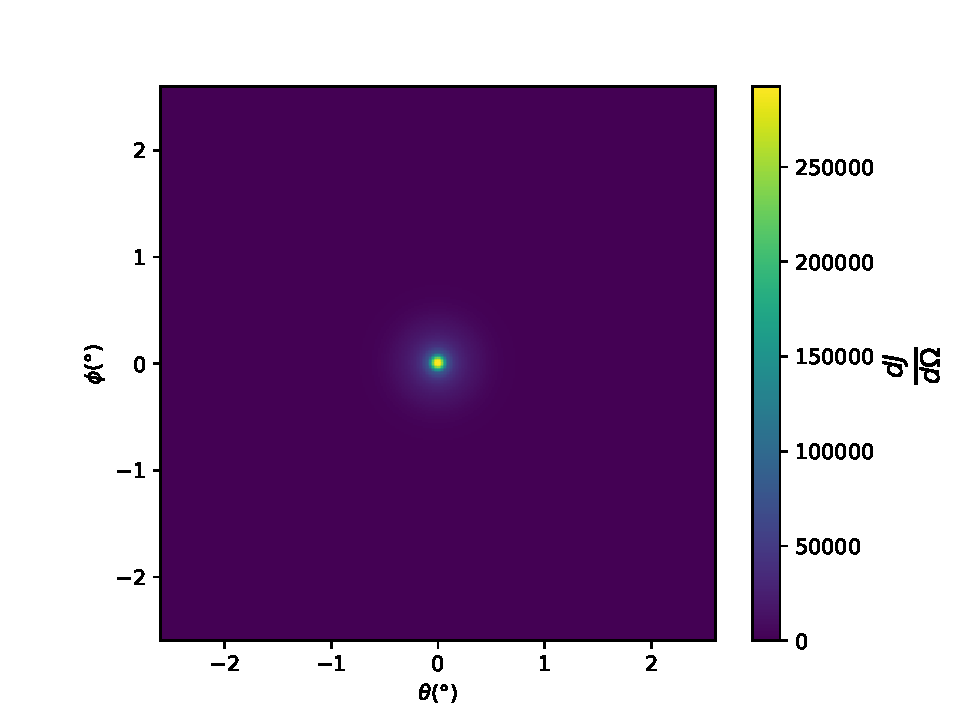
\includegraphics[scale=0.275]{figures/mtd_hawc_dm/Sextans_Jm1_plot.pdf}} &
        \raisebox{-.5\height}{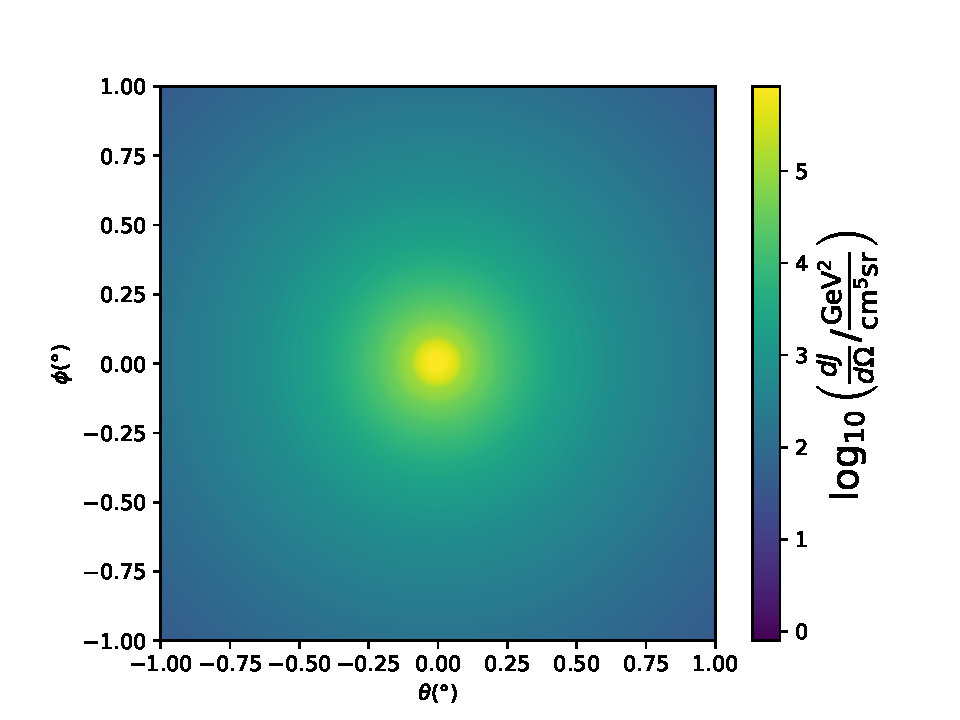
\includegraphics[scale=0.275]{figures/mtd_hawc_dm/Sextans_J_plot.pdf}} &
        \raisebox{-.5\height}{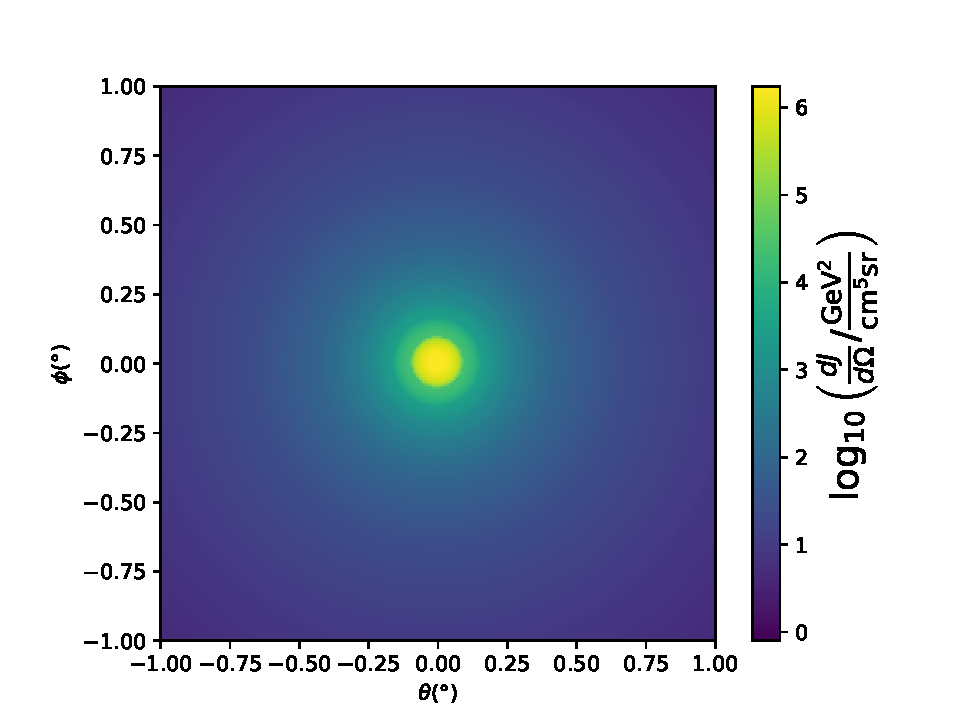
\includegraphics[scale=0.275]{figures/mtd_hawc_dm/Sextans_Jp1_plot.pdf}} \\
    \end{tabular}
    }
    \caption{$\frac{d\J}{d\Omega}$ maps for Coma Berenices, Draco, Segue1, and Sextans. Columns are divided for the $\pm1 \sigma$ uncertainties in $d\J/d\Omega$ around the mean value from \LS \cite{DM_Strigari20}. Origin is centered on the specific dwarf spheroidal galaxies (dSph). $\theta$ and $\phi$ axes are the angular separation from the center of the dwarf}
    \label{fig:ls20_jfac_maps}
\end{figure}

%%%%%%%%%%%%%%%%%%%%%%%%%%%%%%%%%%%%%%%%%%%%%%%%%%
\subsection{Source Selection and Annihilation Channels}\label{sec:mtd_srcs_y_chan}
%%%%%%%%%%%%%%%%%%%%%%%%%%%%%%%%%%%%%%%%%%%%%%%%%%

HAWC's sources for this multithreaded analysis include Coma Berenices, Draco, Segue 1, and Sextans
\LS observes up to 43 sources in its publication, however only 4 of the best fit profiles were provided at the time this thesis was written.
A full description of each source used in this analysis is found in \Cref{tab:mtd_J_factor}.

\begin{table}[b]
\centering
    \small{\begin{tabular}{cccc}
    \hline
    \hline
    \CellTopTwo{}
    Name & Distance & $l, b$ & $\log_{10}J$~(\LS set)\\
    & \scriptsize{(kpc)} &  \scriptsize{($\degree$)} & \scriptsize{$\log_{10}(\mathrm{GeV}^2 \mathrm{cm}^{-5}\mathrm{sr})$} \\
    \hline
    \CellTopTwo{}
    Coma Berenices & $44$ & $241.89,\: 83.61$ & $19.00^{+0.36}_{-0.35}$ \\
    \CellTopTwo{}
    Segue I & $23$ & $220.48,\: 50.43$ & $19.12^{+0.49}_{-0.58}$ \\
    \CellTopTwo{}
    Sextans & $86$ & $243.50,\: 42.27$ & $17.73^{+0.13}_{-0.12}$ \\
    \hline
    \hline
    \CellTopTwo{}
\end{tabular}}
    \caption{Summary of the relevant properties of the dSphs used in the present work. Column 1 lists the dSphs. Columns 2 and 3 present their heliocentric distance and galactic coordinates, respectively. Column 4 reports the \J-factors of each source given from the \LS studies and estimated $\pm 1\sigma$ uncertainties. The values $\log_{10}J$~(\LS set) \cite{DM_Strigari20} correspond to the mean \J-factor values  for a source extension truncated at $0.5^\circ$.}
    \label{tab:mtd_J_factor}
\end{table}

This analysis improves on \Cref{sec:glory_duck} in the following ways.
Previously, the particle physics model used for gamma-ray spectra from DM annihilation was from the PPPC \cite{Cirelli_2011} which missed important considerations relevant for the neutrino sector.
HDM is used to account for this shortfall \cite{HDMSpectra}.
HDM also models DM to the Planck scale which permits HAWC to probe PeV scale DM.
For this study, we sample DM masses: $1$ TeV - $10$ PeV with 6 mass bins per decade in DM mass.
In the case of line spectra ($\chi\chi \rightarrow \gamma\gamma$, or $ZZ$), we double the mass binning to 12 DM mass bins per decade in DM mass.
A larger source catalog is used that uses a Navarro–Frenk–White (NFW) spatial DM distribution from \LS \cite{DM_Strigari20}.
Because NFW has fewer parameters than what is used for \GS, \LS is able to fit ultra-faint dwarves, expanding the number of sources available for DM searches.
Finally, the gamma-ray ray dataset is much larger.
The study performed here analyzes 2565 days of data compared to 1017 days analyzed in \Cref{sec:glory_duck}.

%%%%%%%%%%%%%%%%%%%%%%%%%%%%%%%%%%%%%%%%%%%%%%%%%%%%%%%%%%%%%
\section{Likelihood Methods} \label{sec:mtd_ll_methods}
%%%%%%%%%%%%%%%%%%%%%%%%%%%%%%%%%%%%%%%%%%%%%%%%%%%%%%%%%%%%%

These are identical to \Cref{sec:gd_hawc_llh} and not additional changes are made to the likelihood.
Bins in this analysis are expanded to include HAWC's NN energy estimator.

%%%%%%%%%%%%%%%%%%%%%%%%%%%%%%%%%%%%%%%%%%%%%%%%%%%%%%%%%%%%%
\section{Computational Methods: Multithreading} \label{sec:mtd_comp_methods}
%%%%%%%%%%%%%%%%%%%%%%%%%%%%%%%%%%%%%%%%%%%%%%%%%%%%%%%%%%%%%

Previously, as in \Cref{sec:gd_analysis}, the likelihood was minimized for one model at a time.
One model in this case representing a DM annihilation channel, DM mass, and dSph.
In an effort to conserve human and CPU time, jobs submitted for high performance computing contained a list of DM masses to iterate over for likelihood fitting.
Jobs were then trivially parallelized for each permutation of the two lists: \texttt{CHANS} (SM annihilation channel) and \texttt{SOURCES} (dSph spatial templates).
The lists for \texttt{CHANS} and \texttt{SOURCES} are found in \Cref{sec:mtd_particlephysics} and \Cref{tab:mtd_J_factor}, respectively.
Initially, 11 DM mass bins were serially sampled for one job defined by a [SM channel, dSph] set.
Computing the likelihoods would take between 1.5 to 2 hrs, stocastically, for a job.
We expect to compute likelihoods for data and 300 Poisson background trials.
The estimated CPU time based on the above for all SM annihilation channels (17) and 25 sources (all \LS sources withing HAWC's field of view) amounted to $127,925$ jobs.
In total, $1,407,175$ likelihood fits and profiles would be computed for the 11 mass bins we wished to study.
The estimated CPU time ranged between $10$k CPU days - $8$k CPU days.
Human time is more challenging to estimate as job allocation is stocastic and highly dependant on what other users are submitting, yet it is unlikely that all jobs would run simultaneously.
Therefore we can expect human time to be about as long as was seen in \Cref{sec:glory_duck} which was on the order of months to fully compute on a smaller analysis.
A visual aid to describe how jobs were organized is provided in \Cref{fig:mtd_gd_workflow}.

\begin{figure}[h]
    \centering{
        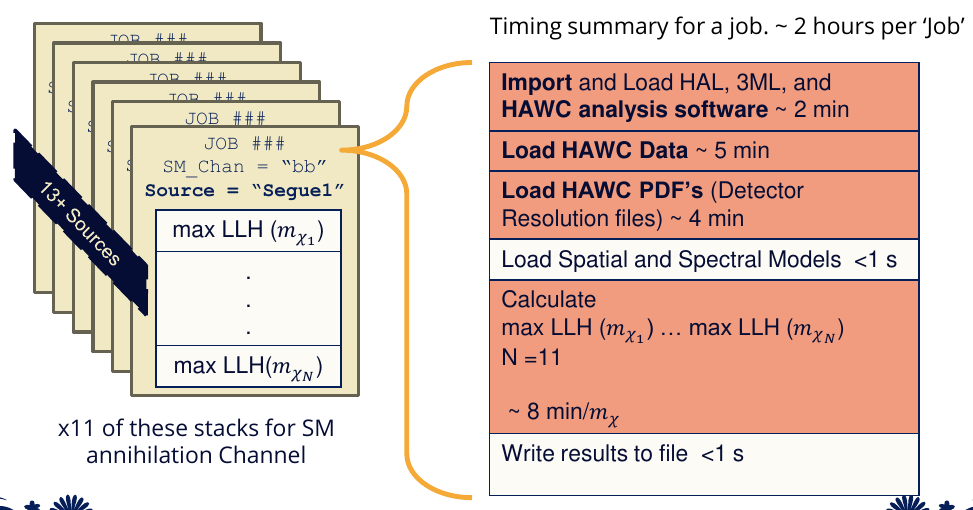
\includegraphics[scale=0.6]{figures/mtd_hawc_dm/gd_workflow.png}
    }
    \caption{Infographic on how jobs and DM computation was organized in \Cref{sec:gd_analysis}. Jobs were built for each permutation of \texttt{CHANS} and \texttt{SOURCES} shown by the left block in the figure. Each job, which took on the order 2 hrs to compute, had the following work flow: 1. Import HAWC analysis software, 2 min to run. 2. Load HAWC count maps, 5 min to run. 3. Load HAWC energy and spatial resolutions, 4 min. 5. Load DM spatial source templates and spectral models, less than 1 s. 6. Perform likelihood fit on data and model, about 8 min per DM mass. 7. Write results to file, less than 1s.}
    \label{fig:mtd_gd_workflow}
\end{figure}


The computational needs for this next generation DM analysis are extreme and is unlike other analyses performed on HAWC.
It became clear that there was a lot to gain from optimzing how the likelihoods are computed.
This section discusses how multi-threading was applied to solve and reduce HAWC's computing of likelihoods for large parameter spaces like in DM searches.

%%%%%%%%%%%%%%%%%%%%%%%%%%%%%%%%%%%%%%%%%%%%%%%%%%%%%%%%%%%%%
\subsection{Relevant Foundational Information}\label{sec:mtd_foundation}
%%%%%%%%%%%%%%%%%%%%%%%%%%%%%%%%%%%%%%%%%%%%%%%%%%%%%%%%%%%%%

The profiling of the likelihood for HAWC is done via gradient descent where the nomarlization of \Cref{eq:id_dm_flux} (linearly correlated with \sv) is rescaled in the descent.
Additionaly, we sample the likelihood space for a defined list of \sv's described in \Cref{sec:gd_joint_llh}.
The time to compute these values is not predictable or consistent because many variables can change across the full model-space.
comprehensively, these variables are:
\begin{itemize}
    \item $m_\chi$ : DM rest mass
    \item \texttt{CHAN} : DM SM annihilation channel.
    \item \texttt{SOURCE} : dSph within HAWC's field of view. This involves a spatial template AND coordinate in HAWC data.
    \item \sv~: Effectevly the flux normalization and free parameter in the likelihood fit.
\end{itemize}
Therefore, we develop an asyncronous, functional-parallel coding pattern.
Asyncronous meaning that the instructions and computing within a function are independent and permitted to be out of sync with sibling computations.
Functional-parallel meaning that instructions are the subject of parrallelization rather than threading the likelihood computation.
This is close to trivial parametrization seen in \Cref{fig:mtd_gd_workflow} except that we seek to consolidate the loading stages (software, data, and detector resolution loading).
Reducing the total instances of loading stages and distributing access to the reduced loads across multiple asyncronous threads is expected to reduce serial processing time and the overhead implicit to each job in addition to saving human time.

\begin{figure}[h]
    \centering{
        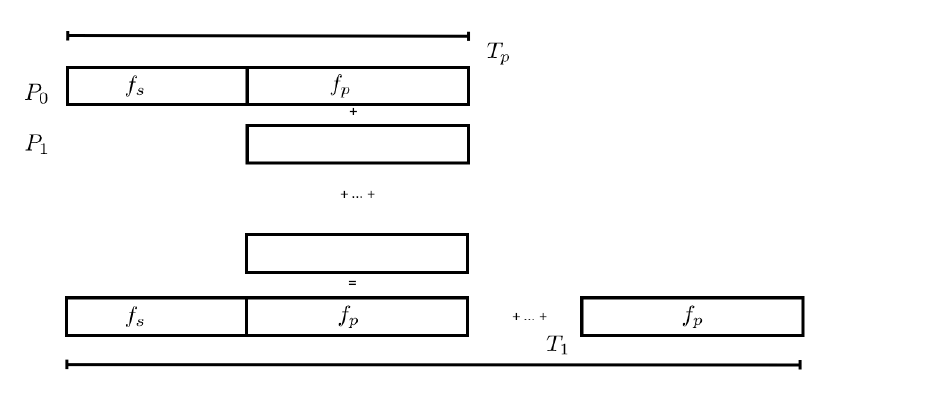
\includegraphics[scale=0.65]{figures/mtd_hawc_dm/gufstafson_coding_pattern.png}
    }
    \caption{Graphic of Gustafson parallel coding pattern. $f_s$ is the fraction of a program, in time, spent on serial computation. $f_p$ is the fraction of computing time that is parallelizable. $T_p$ is the total time for a parallel program to run. $T_1$ is the total time for a parallel program to run if only 1 processor is allocated. $P_N$ is the $N$-th processor where it's row is the computation the processor performs. The Gustafson pattern is most similar to what is implemented for this analysis. Figure is pulled from \cite{ArtofHPC}.}
    \label{fig:mtd_gufsta}
\end{figure}

We need a way to measure and compare the expected speedup and efficiency gain for this asyncronous coding pattern.
I pull inspiration for timing measurement from \cite{ArtofHPC} and use \textit{Amdahl's law with hybrid programming}.
Hybrid programming meaning that the computation is a mix of distributed and shared memory programming.
If we assume the code is fully parallelizable over $p$ processors and $c$ threads, the ideal speedup is simply $pc$ and ideal run-time is $T_1/(pc)$.
$T_1$ is the total time for a parallel program to run if only 1 processor is allocated.
However, the coding pattern contains some amount of unavoidable serial computation, as shown in \Cref{fig:mtd_gufsta}.
In our case, the run time is estimated to be
\amdahl
$F_s$ is the fraction of CPU time dedicated to serial computation.
The expected speedup is
\amdahlSpeed
From \Cref{eq:amdahlSpeed}, we can see that the speed up scales with $p/F_s$.
We are free to minimize $F_s$ asymptotically by enlarging the total models that are submitted to the thread pool, thereby shrinking the CPU fraction dedicated to serial operation.
We are also free to define exactly how many threads and processors we utilize, yet eventually hit a hard cap at the hardware available on our computing cluster.
HAWC uses Intel Xeon processors with 48 cores and 96 threads.
This means when N-threads ($c$) are defined, N mod 2 cores ($p$) are needed.
We see that a successful code scales well as the expected speedup is inversely correlated with $F_s$.
As the total number of models sampled grows, the speedup will also.

%%%%%%%%%%%%%%%%%%%%%%%%%%%%%%%%%%%%%%%%%%%%%%%%%%%%%%%%%%%%%
\subsection{Implementation}\label{sec:mtd_implementation}
%%%%%%%%%%%%%%%%%%%%%%%%%%%%%%%%%%%%%%%%%%%%%%%%%%%%%%%%%%%%%

\begin{figure}[h]
    \centering{
        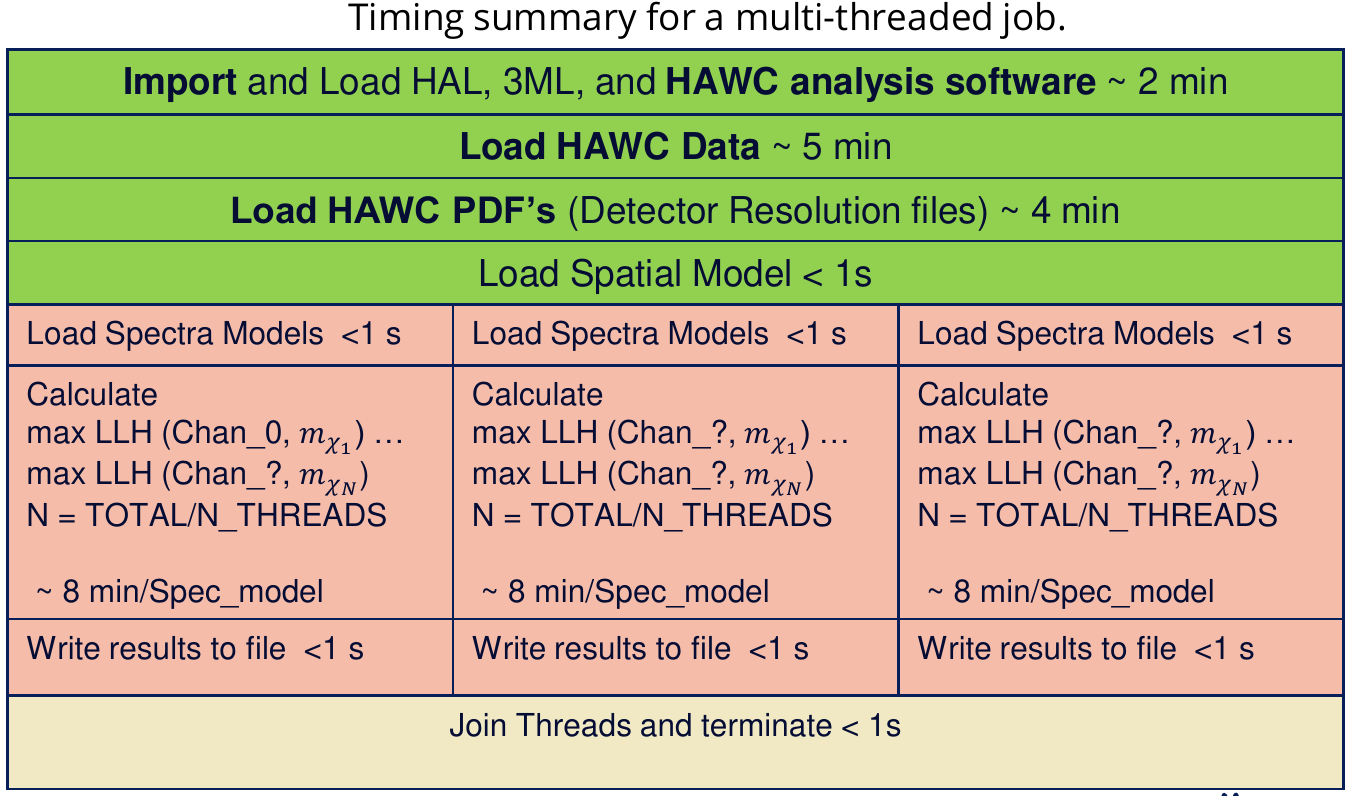
\includegraphics[scale=0.4]{figures/mtd_hawc_dm/mult-threaded_hawc.png}
    }
    \caption{Task chart for one multi-threaded job developed for this project. Green blocks indicate a shared resource across the threads AND computation performed serially. Red blocks indicate functional parallel processing within each thread. 3 threads are represented here, yet many more can be employed during the full analysis. Jobs are defined by the \texttt{SOURCE} as these require unique maps to be loaded into the likelihood estimator. The $m_\chi$, \texttt{CHAN}, and \sv~variables are entered into the thread pool and allocated as evenly as possible across the threads.}
    \label{fig:mtd_multithreads}
\end{figure}

The multithreaded code was written in Python3 and is documented in the \texttt{dark\_matter\_hawc} \href{https://gitlab.com/hawc-observatory/sandboxes/salaza82/dark\_matter\_hawc}{repository} within the script named \texttt{mpu\_analysis.py}.
A version of the script as of April 25 \todo{make sure to update on this date} is also provided in \Cref{sec:apx_mpu_script}
It has many dependancies including the HAWC analysis software.
\Cref{fig:mtd_multithreads} displays the workflow of a job with 3 threads.
Within a job, \texttt{SOURCE} is kept fixedh .
\texttt{CHAN(S)} remains 17 elements long.
More $m_\chi$ are sampled from 11 bins up to 49 (for $\gamma\gamma$ and $ZZ$) and 25 (for remaining \texttt{CHANS}) which amounts to 12 or 6 mass bins per decade.
The DM mass, $m_\chi$, and SM annihilation channels, \texttt{CHANS}, are permuted into a 473 element list which is split evenly across N threads where N ranges between 5 - 16.
Within a thread, for each $m_\chi$-\texttt{CHAN} tuple, 1001 \sv~values are sampled in the likelihood, and the value of \sv~that maximizes the likelihood is found.
Although rare, fits that failed are handled on a case by case basis.

%%%%%%%%%%%%%%%%%%%%%%%%%%%%%%%%%%%%%%%%%%%%%%%%%%%%%%%%%%%%%
\subsection{Performance}\label{sec:mtd_performance}
%%%%%%%%%%%%%%%%%%%%%%%%%%%%%%%%%%%%%%%%%%%%%%%%%%%%%%%%%%%%%

\begin{table}[h]
    \centering
    {\begin{tabular}{c ? c  c  c  c }
    & \multicolumn{4}{c}{$T_{p,c}$ (hr:min:s)} \\
    \hline
    \hline
    M Tasks & $T_{1,1}$ & $T_{1,2}$ & $T_{1,8}$ & $T_{1,16}$ \\
    \hline
    50 & 1:40:37.5 & 0:52:43.7 & 0:19:13.8 & 0:13:44.0 \\
    74 & 2:22:30.0 & 1:15::00.6 & 0:25:21.3 & 0:15:49.8 \\
    100 & (3:07:51.9) & 1:40:10.5 & 0:30:44.4 & 0:20:01.4 \\
    200 & (6:02:20.6) & - & &  \\
    473 & (13:58:40.3) & - & & 1:09:42.9 \\
    \end{tabular}}
    \caption{ Timing summaries for analyses for serial and multithreaded processes. M tasks is the number of functional-parallel tasks ran for the computation. $T_{p,c}$ is a single run time in hours:minutes:seconds for runs utilizing $p$ nodes and $c$ threads. Runs are run interactively on the same computer to maximize consistency. Empty entries are indicated with '-'. $(\cdot)$ entries are estimated entries extrapolated from data earlier in the column.}\label{tab:mtd_timing_study}
\end{table}

We see a tremendous reduction to human time waiting for our dSph analyses to run.
\Cref{tab:mtd_timing_study} shows the timing summaries for analyses of different sizes and thread counts.
Additionaly, the efficiency gained when consolidating the serial loading of data is also apparent in our ability to study many more tasks in about the same amount of wall time as a smaller serial computation.
Trials represented in the table were run on an AMD Opteron\textsuperscript{\textregistered} processor 6344 with 48 cores, 2 threads per core; 2.6 GHz clock.
This is not the same architecture used for analysis on the computing cluster however they are similar enough that results shown here are reasonably representative of computing on the HAWC computing cluster.
I use the \cref{tab:mtd_timing_study} for the inferences and conclusions in the following paragraphs.

First, we want to find $T_s$, the time of serial computation.
From \cref{fig:mtd_gufsta}, the timing for our coding pattern can be written as
\TimingAll
$M$ is the number of functional-parallel tasks (represented as column 1 of \cref{tab:mtd_timing_study}), and $t_p$ is the average time to complete a single parallel task.
$T^M_{1,1}$ is the total time for a parallel program to run if only 1 processor is allocated for M parallel task.
With two runs of different M ($M1$ and $M2$), we can use a system of equations to derive
\TsfromMs
We also extract $t_p$ using the same methods:
\TpfromMs
From \cref{tab:mtd_timing_study}, we set $M1 = 50$ and $M2 = 74$ and take their corresponding $T_{1,1}$ from the table to calculate $T_s$ and $t_p$.
\TsTp{803.1}{104.6}
Now, we have specific estimation for the fraction of serial computing time, $F_s$:
\specificFs{803.1}{104.6}
The maximum M for this study is 473 which evaluates \cref{eq:specificFs}: $F_s = 0.016$ or 1.6\% of computing time.
\Cref{tab:mtd_speedup_study} shows the resulting speedups.
\begin{table}[h]
    \centering
    {\begin{tabular}{c c ? c c c}
    & \multicolumn{3}{c}{$S_{p,c}$} \\
    \hline
    \hline
    M Tasks & $F_s$ & $S_{1,2}$ & $S_{1,8}$ & $T_{1,16}$ \\
    \hline
    50  & & 1.90 [1.76] & 5.23 [4.14] & 6.35 [5.34] \\
    74  & & 1.90 [1.83] & 5.62 [4.82] & 9.00 [6.64] \\
    100 & & & & \\
    200 & & - & & \\
    473 & & - & & 1:09:42.9 \\
    \end{tabular}}
    \caption{ Speed up summaries for analyses for serial and multithreaded processes. M tasks is the number of functional-parallel tasks ran for the computation. $S_{p,c}$ is a single speedup comparison for runs utilizing $p$ nodes and $c$ threads. $[\cdot]$ are the estimated speedups calculated from \cref{tab:mtd_timing_study}, \cref{eq:specificFs}, and \cref{eq:amdahlSpeed}. Empty entries are indicated with '-'.}\label{tab:mtd_speedup_study}
\end{table}

We see a speedup that exceeds expectations from \cref{eq:amdahlSpeed} for real trail runs.
\todo{reflect on results when the tables are totally filled in.}
We also see that there are diminishing returns as the number of threads increases.
For small jobs with large $c$, both the expected and observed speedup are significantly smaller than $c$.
One thing not considered in \cref{eq:amdahlSpeed} is the time incurred via communication latency.
Communication latency increases with the number of threads and contributes to diminishing returns.
Therefor, these results are not conclusive.
Each entry in \cref{tab:mtd_timing_study} represent only one run of the script and therefore the data are not precise and lacks the full scope of timing costs.
Yet, they do give us a good idea of what HAWC gains in multithreading analysis software.
We see very clearly that there is a lot to gain, and this new coding pattern will expand HAWC's analysis capabilities.

%%%%%%%%%%%%%%%%%%%%%%%%%%%%%%%%%%%%%%%%%%%%%%%%%%%%%%%%%%%%%
\section{Analysis Results}\label{sec:mtd_results}
%%%%%%%%%%%%%%%%%%%%%%%%%%%%%%%%%%%%%%%%%%%%%%%%%%%%%%%%%%%%%

\begin{figure}[h]
\centering{
    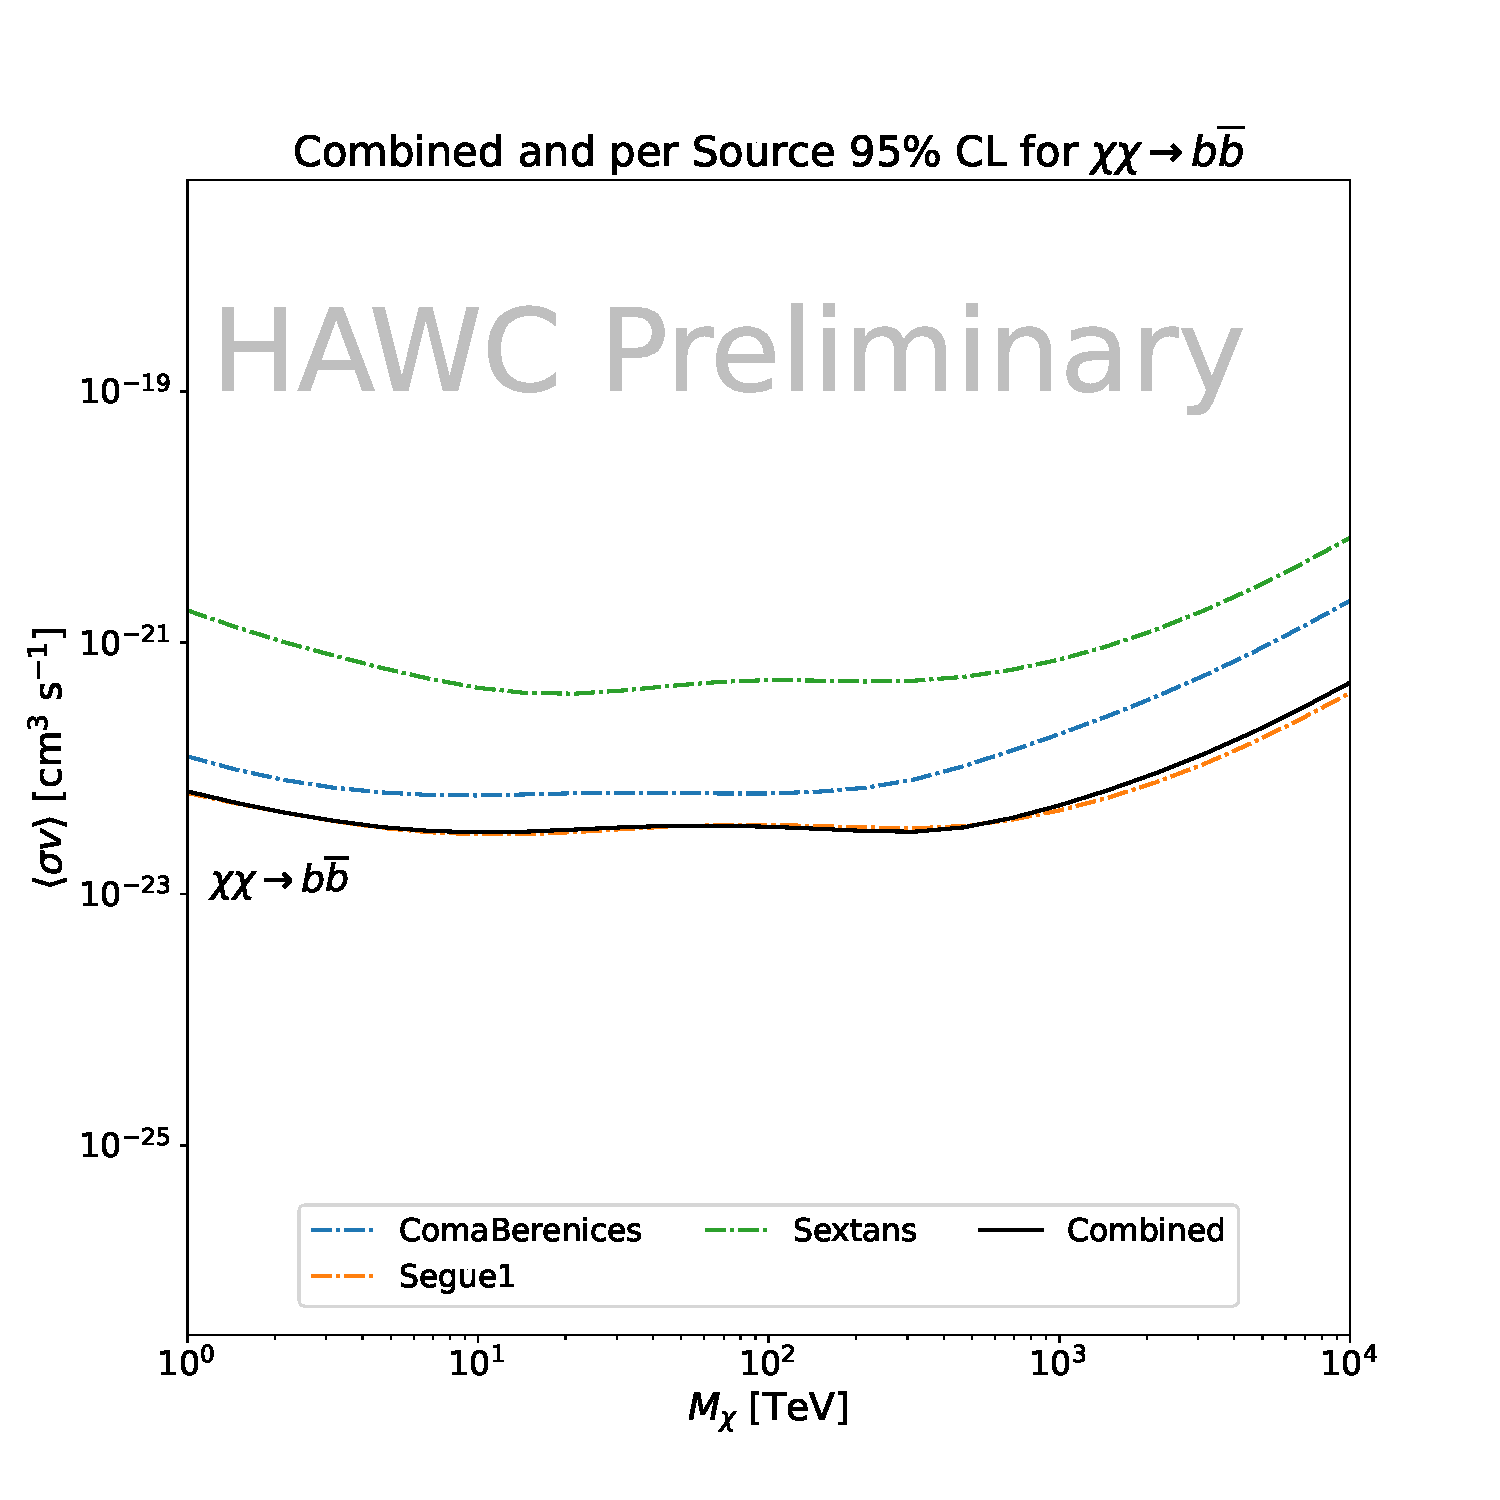
\includegraphics[scale=0.21]{figures/mtd_hawc_dm/results/Combined95_New_duck_bb_.pdf}
    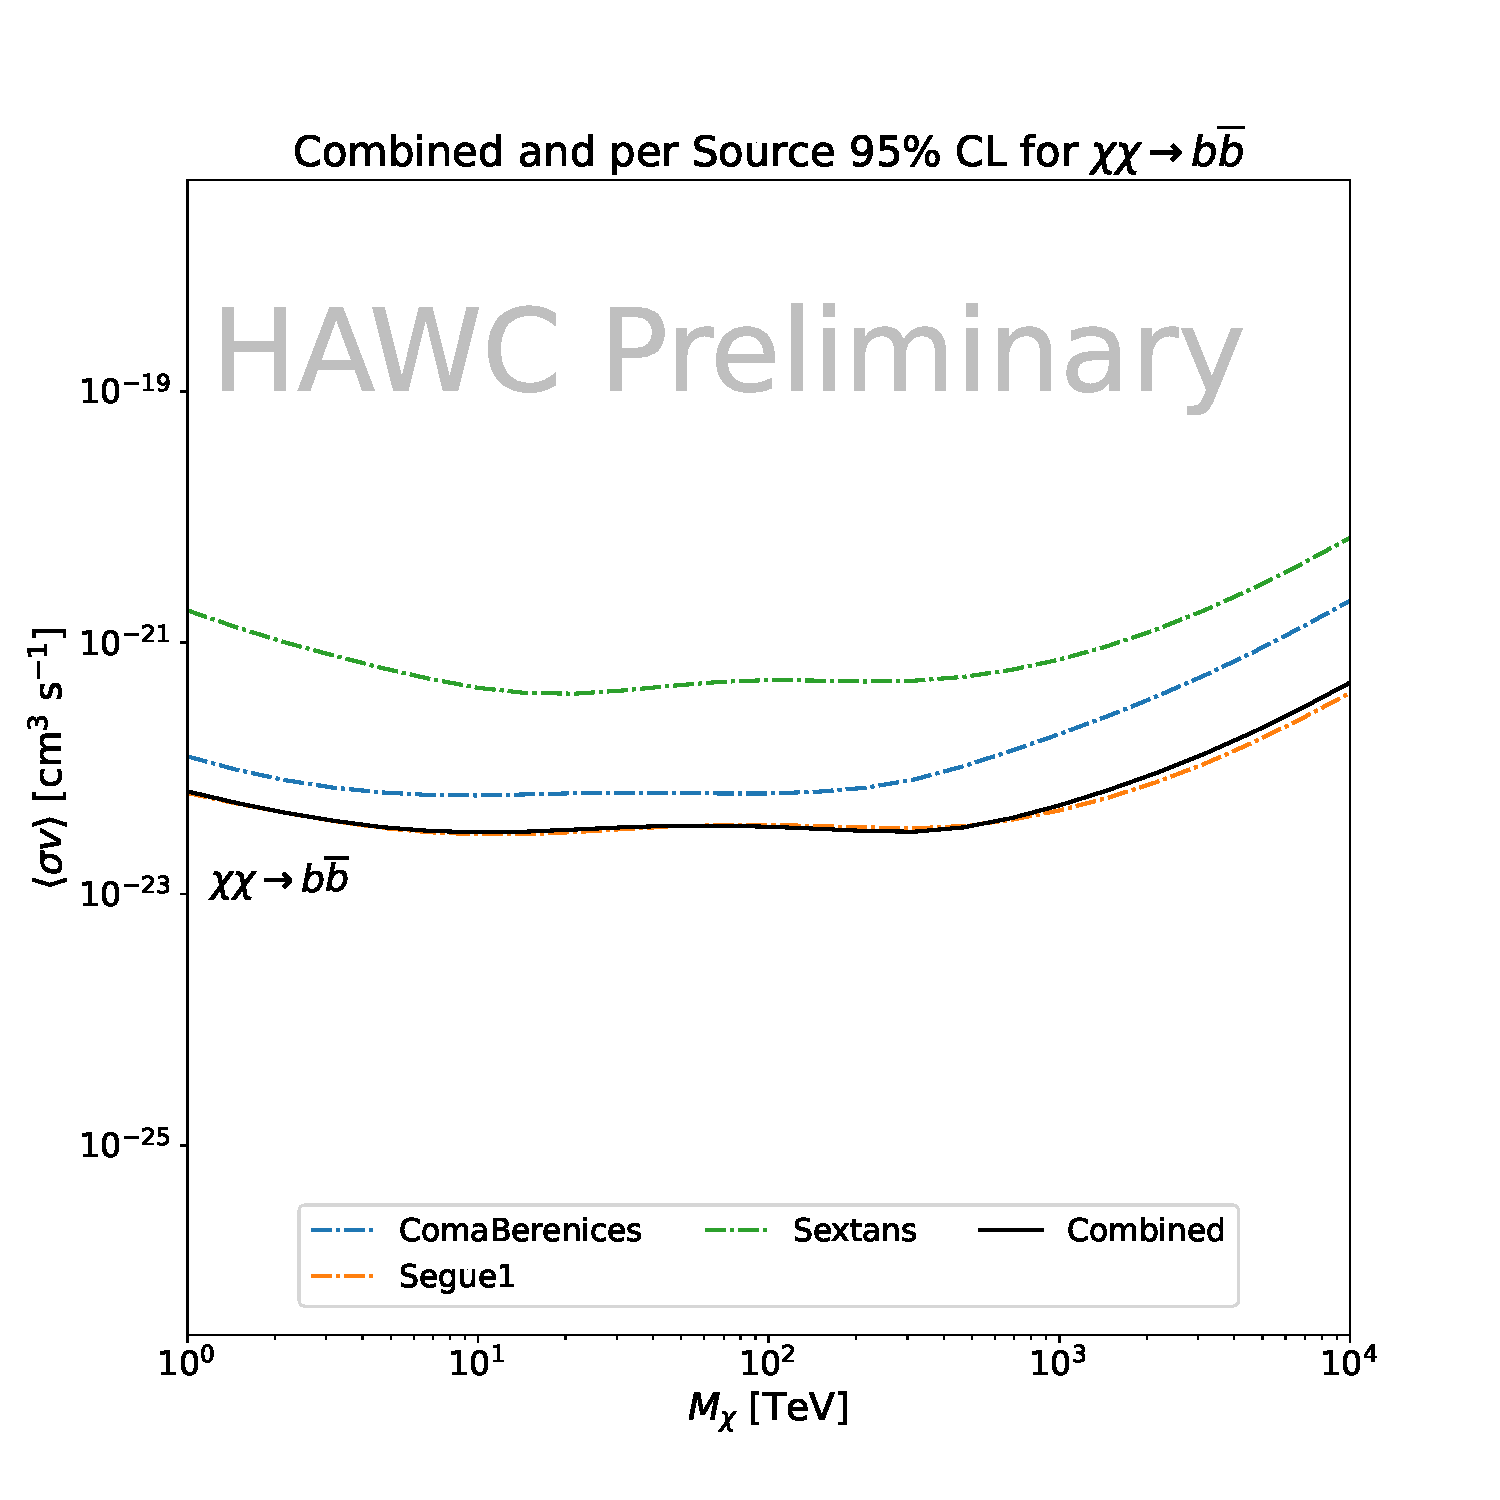
\includegraphics[scale=0.21]{figures/mtd_hawc_dm/results/Combined95_New_duck_bb_.pdf}
    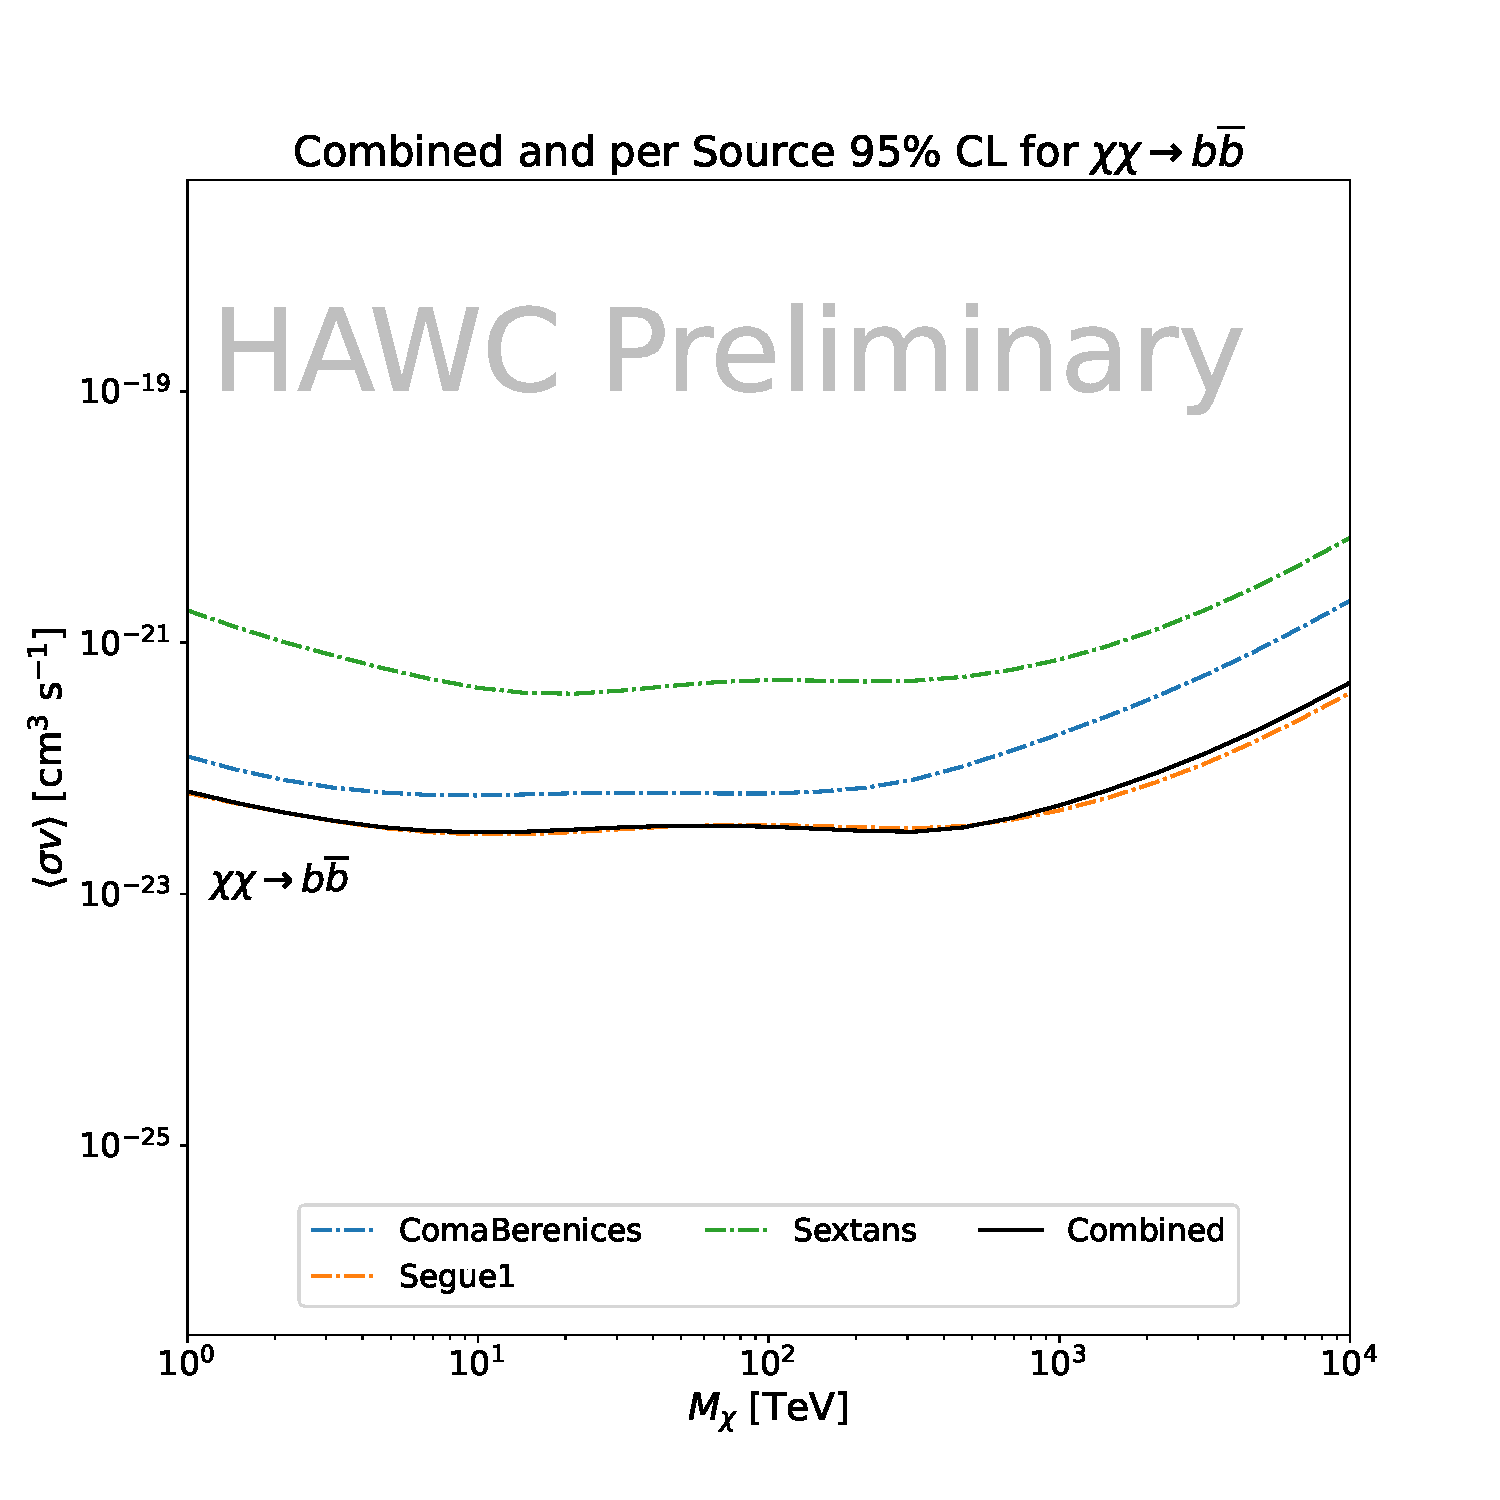
\includegraphics[scale=0.21]{figures/mtd_hawc_dm/results/Combined95_New_duck_bb_.pdf}
    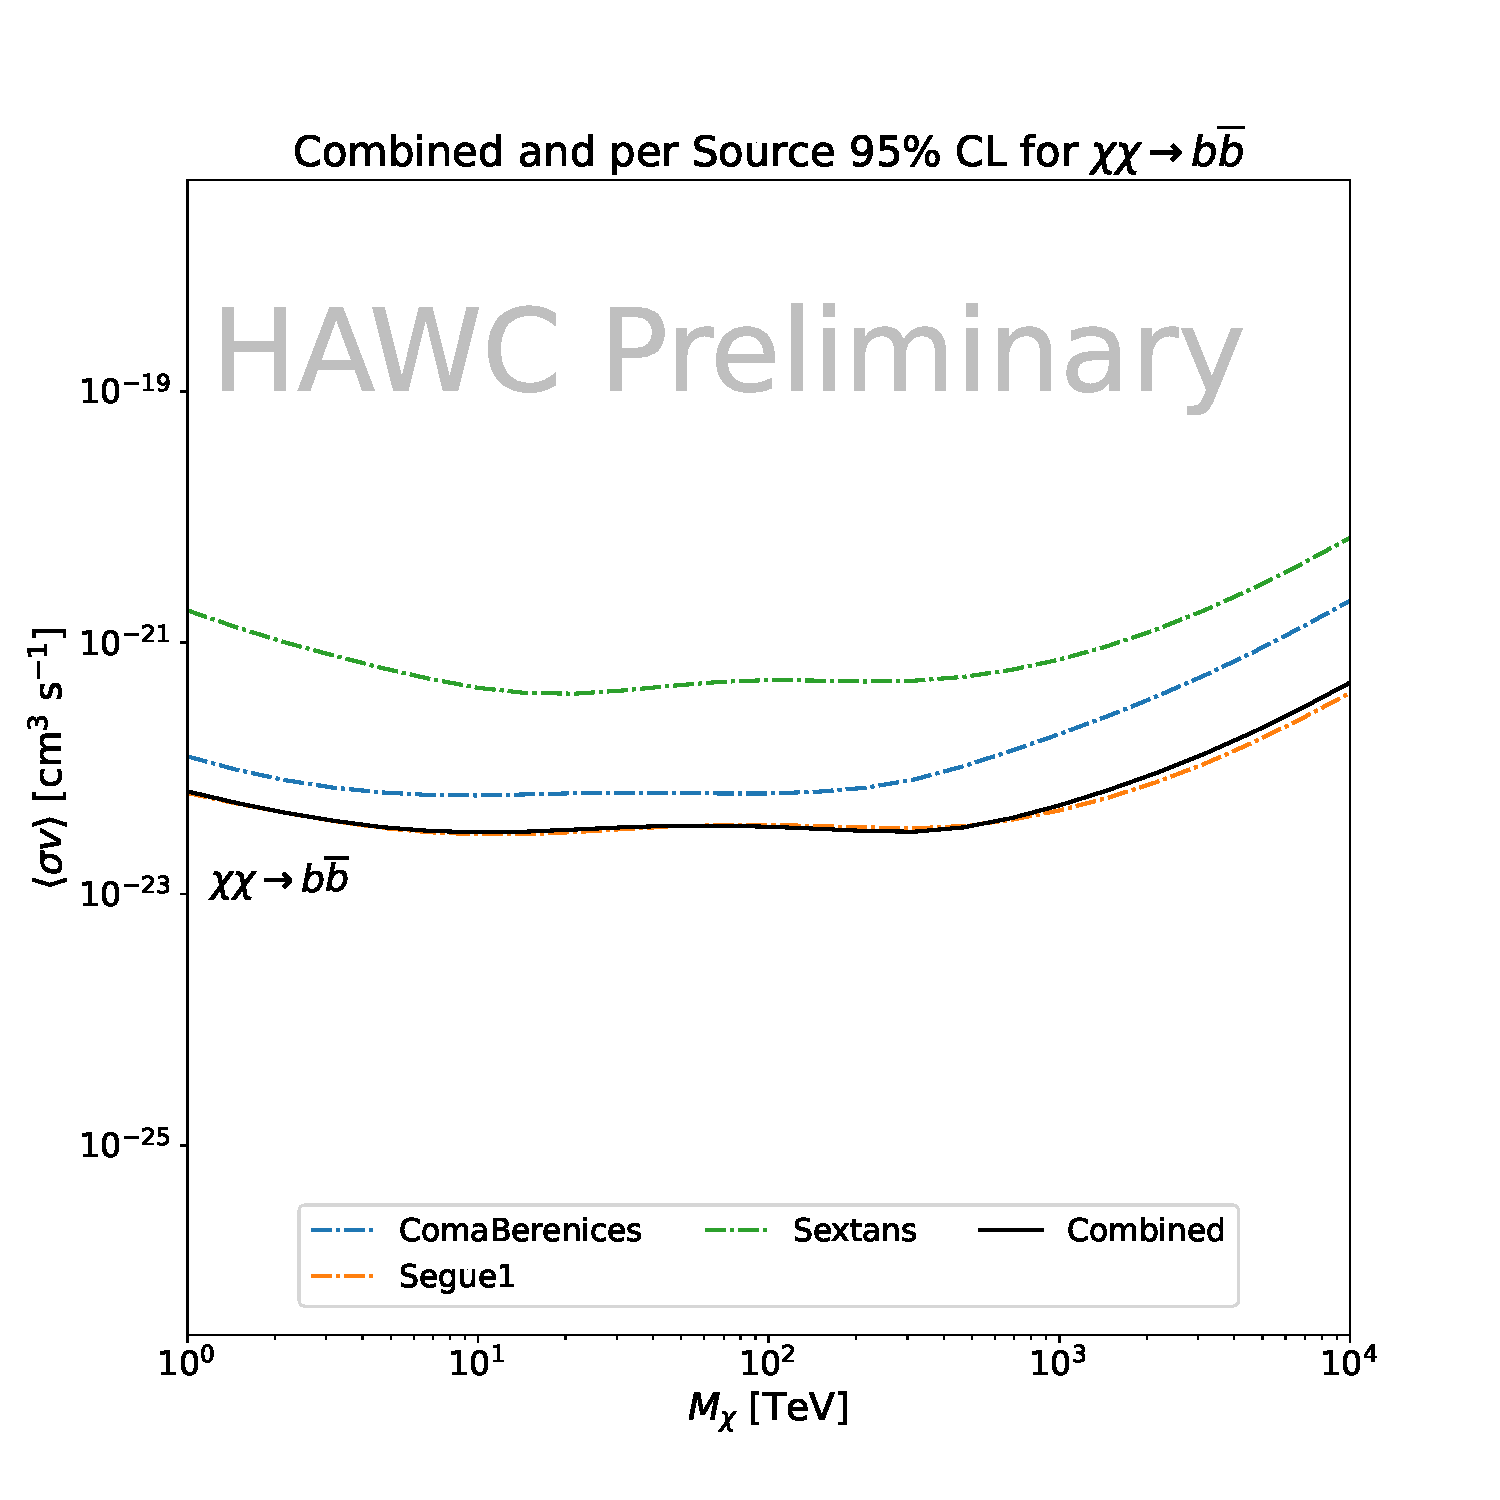
\includegraphics[scale=0.21]{figures/mtd_hawc_dm/results/Combined95_New_duck_bb_.pdf}
    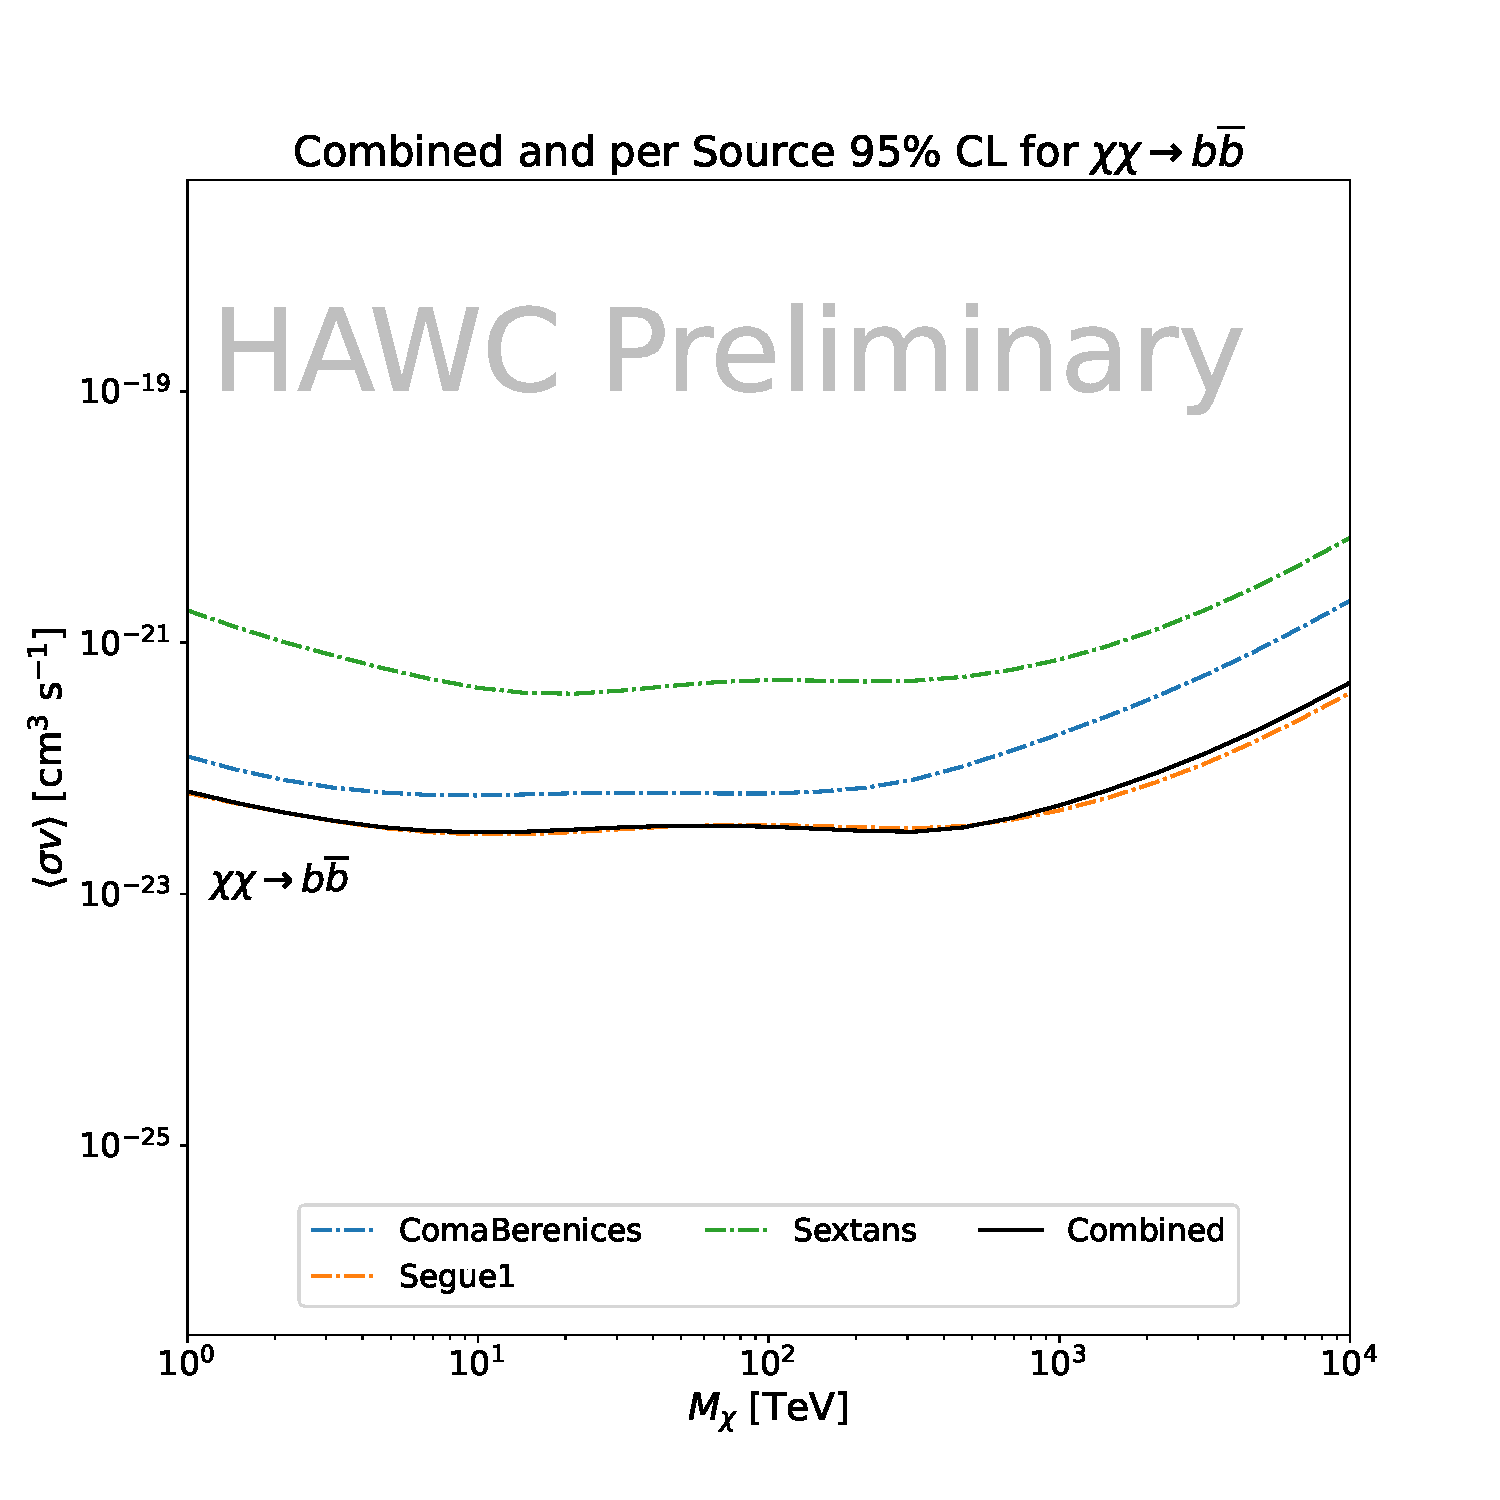
\includegraphics[scale=0.21]{figures/mtd_hawc_dm/results/Combined95_New_duck_bb_.pdf}
    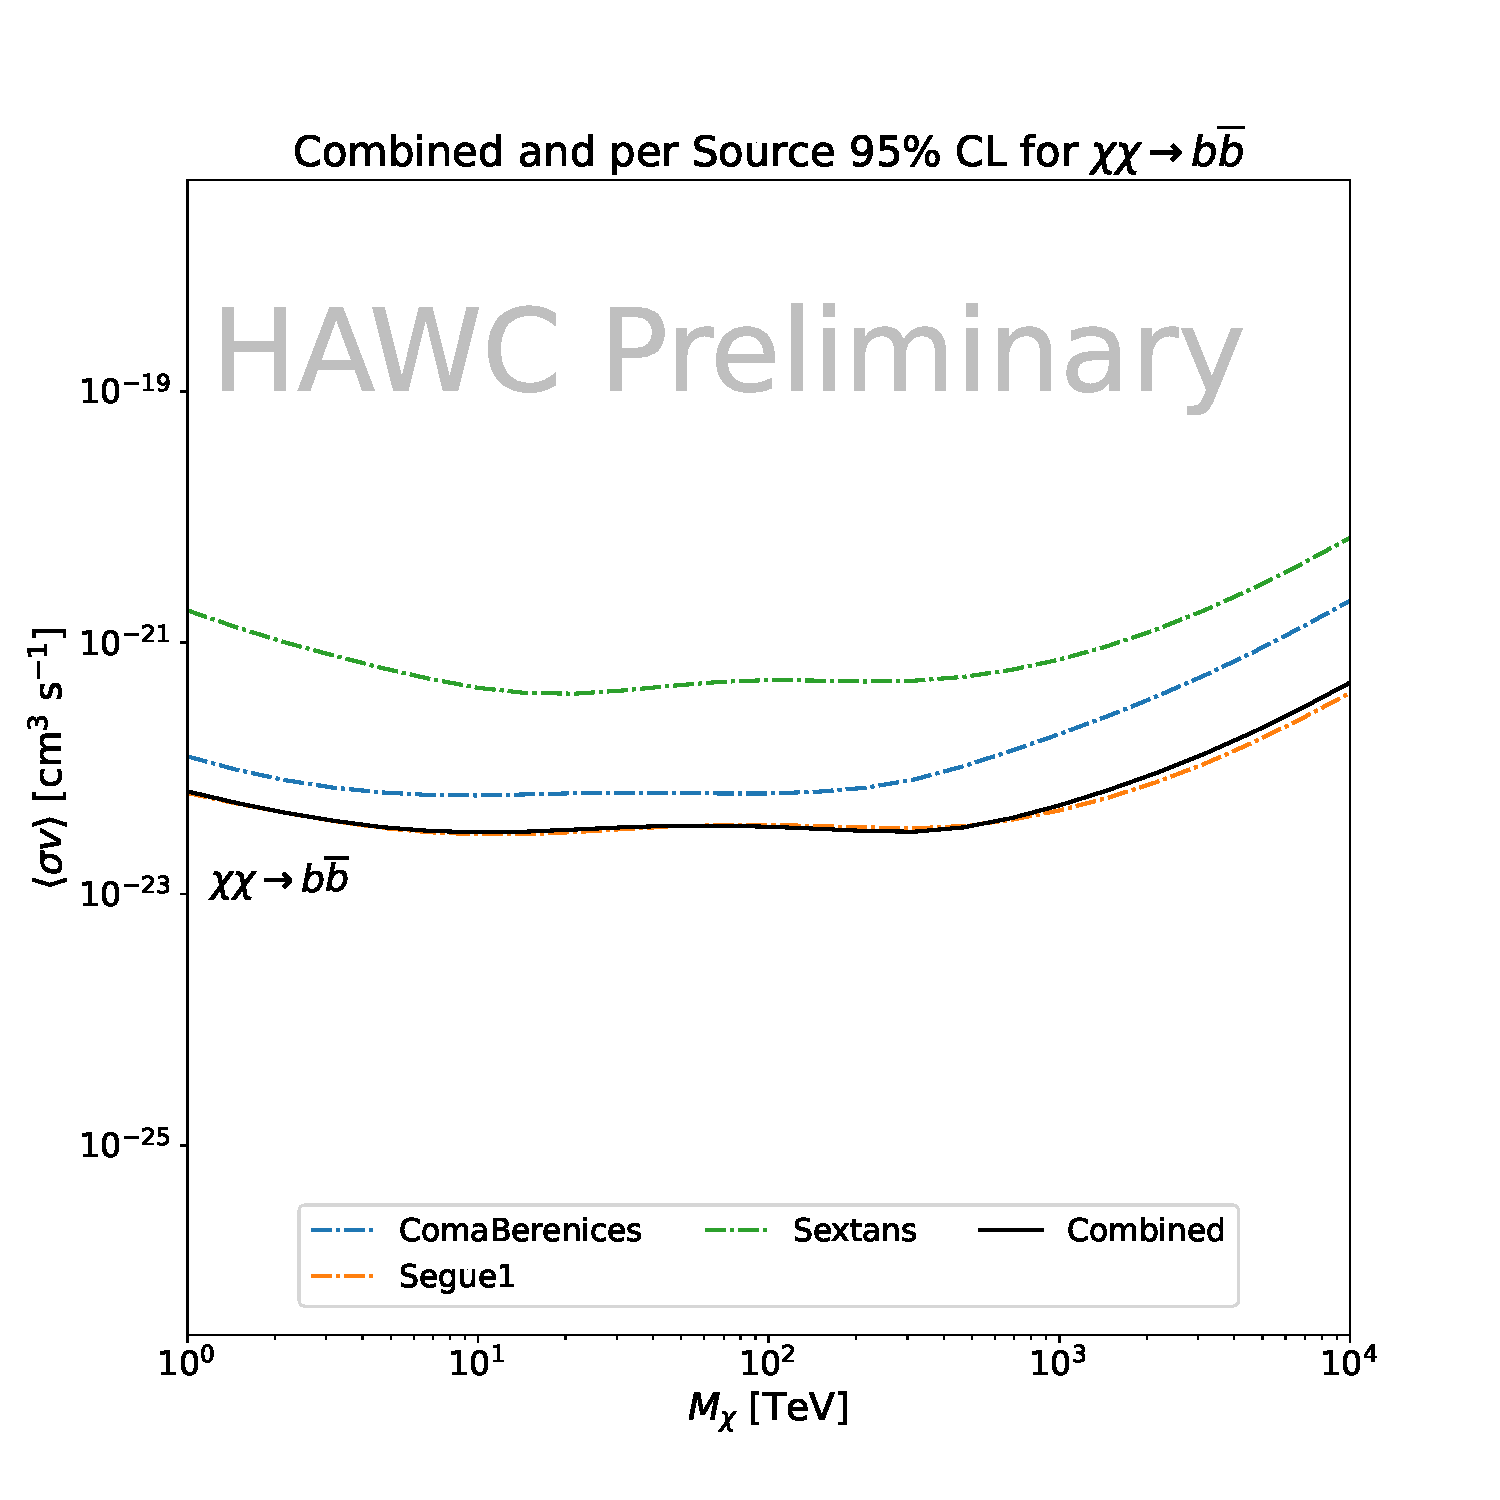
\includegraphics[scale=0.21]{figures/mtd_hawc_dm/results/Combined95_New_duck_bb_.pdf}
    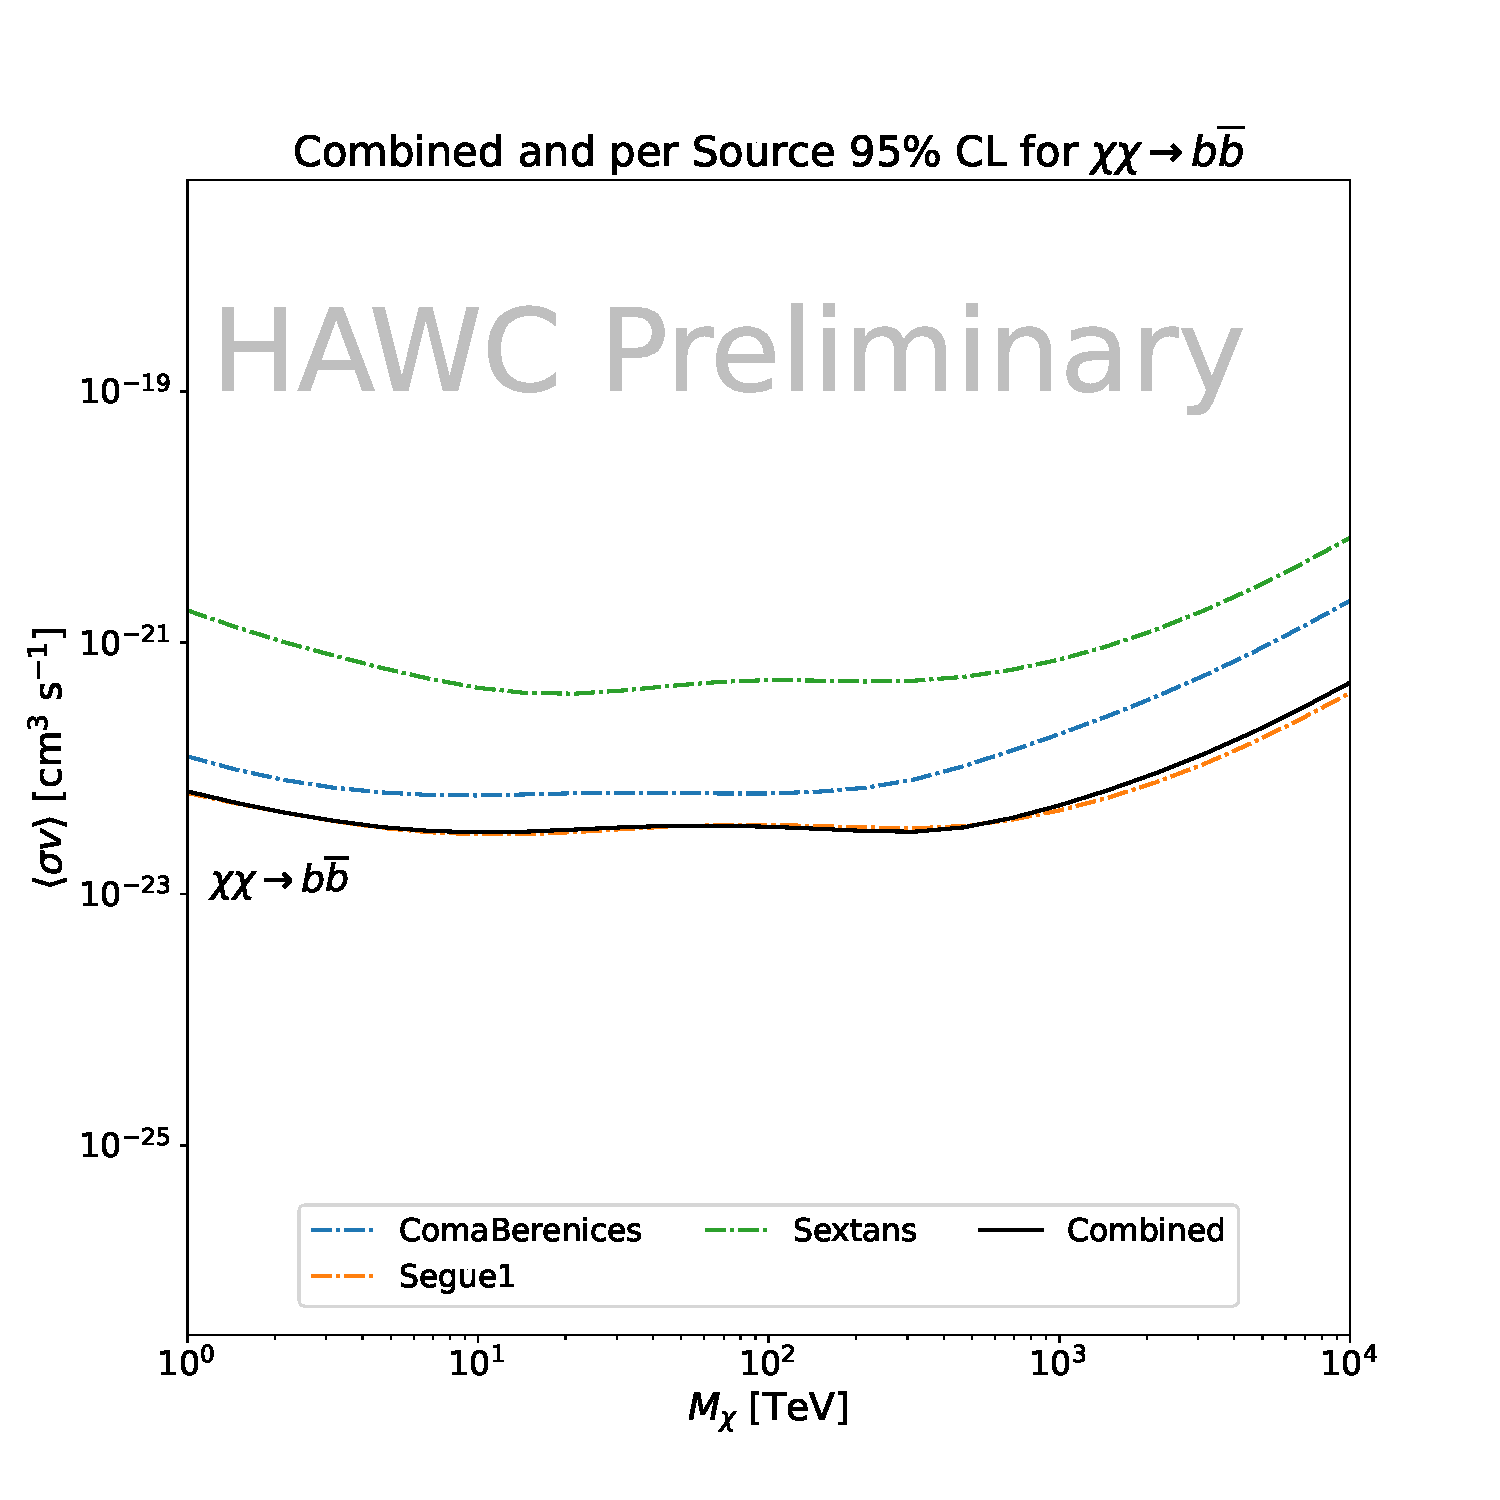
\includegraphics[scale=0.21]{figures/mtd_hawc_dm/results/Combined95_New_duck_bb_.pdf}
    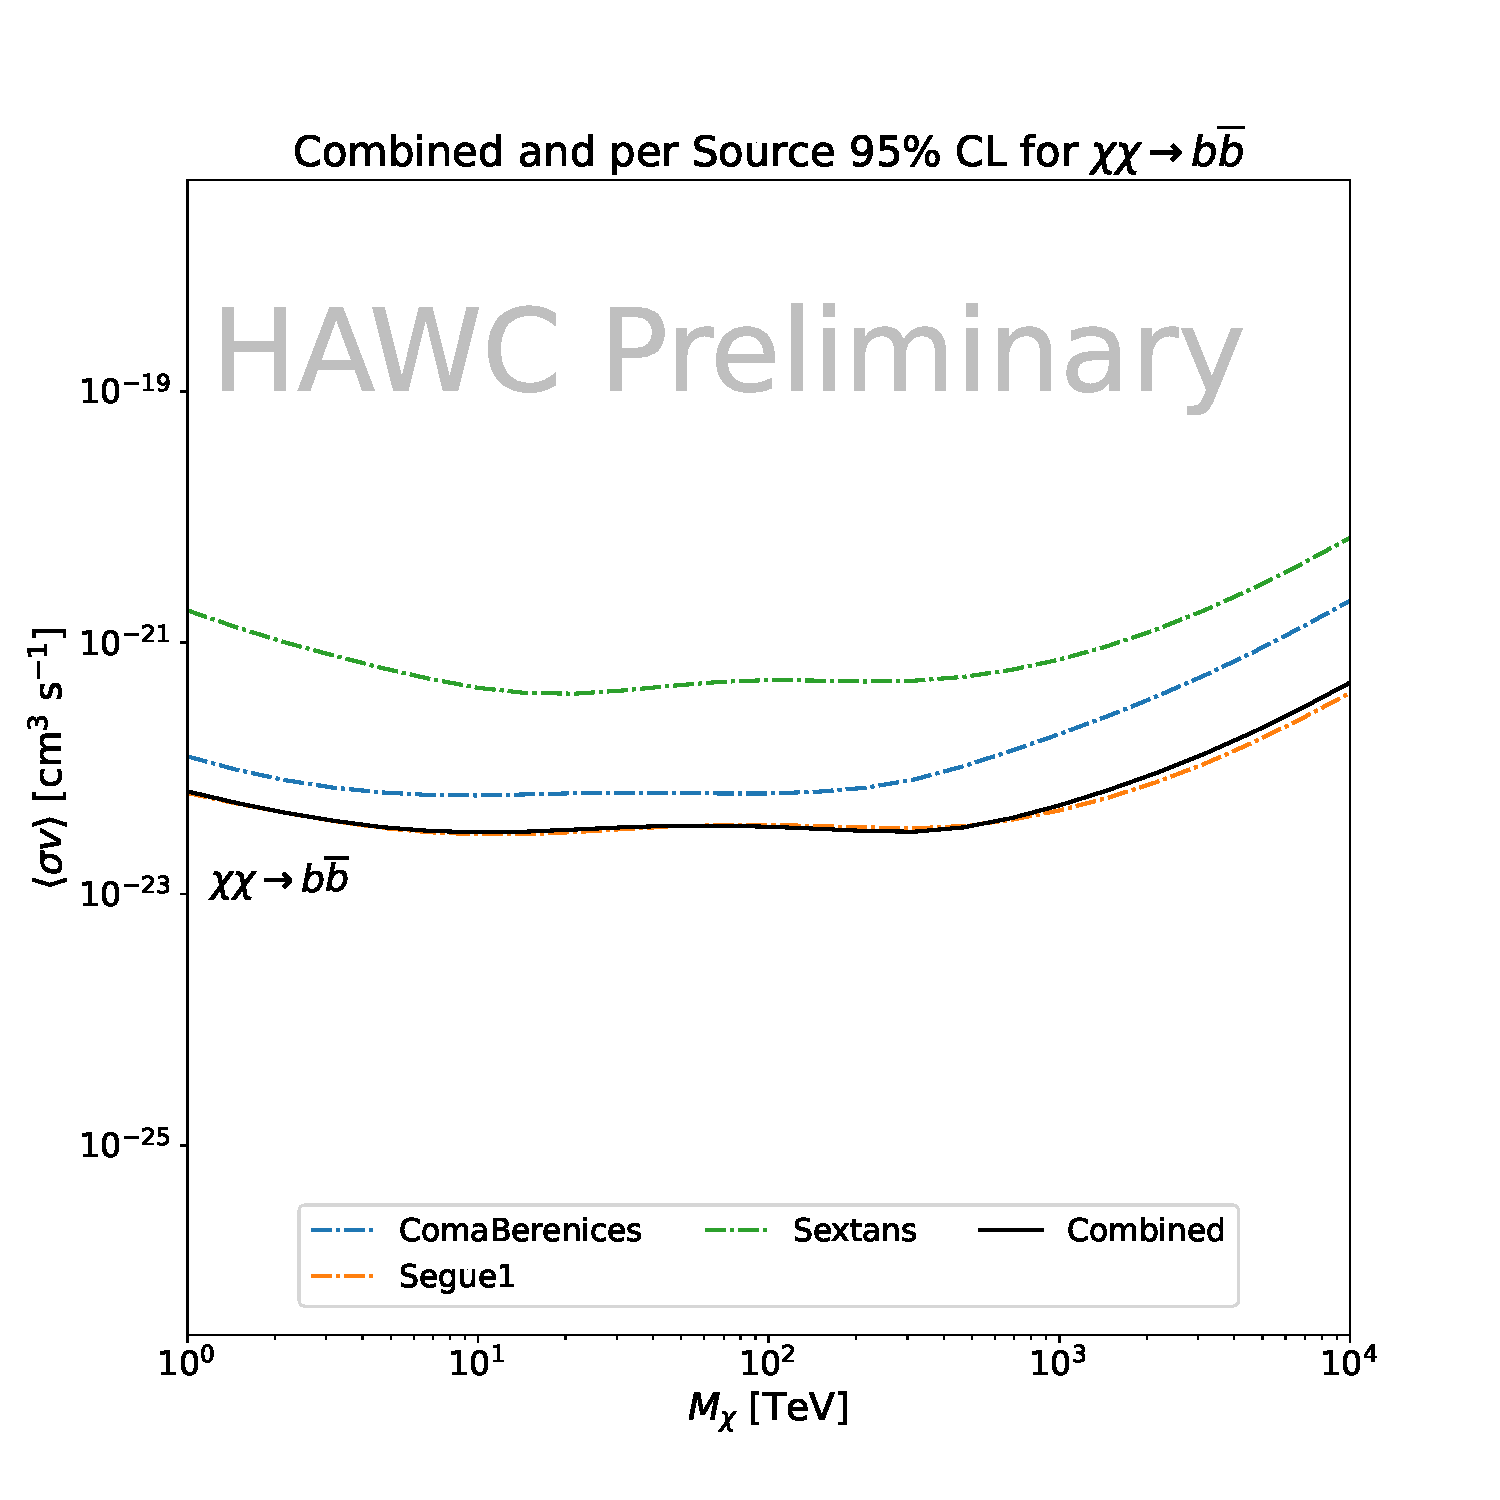
\includegraphics[scale=0.21]{figures/mtd_hawc_dm/results/Combined95_New_duck_bb_.pdf}
    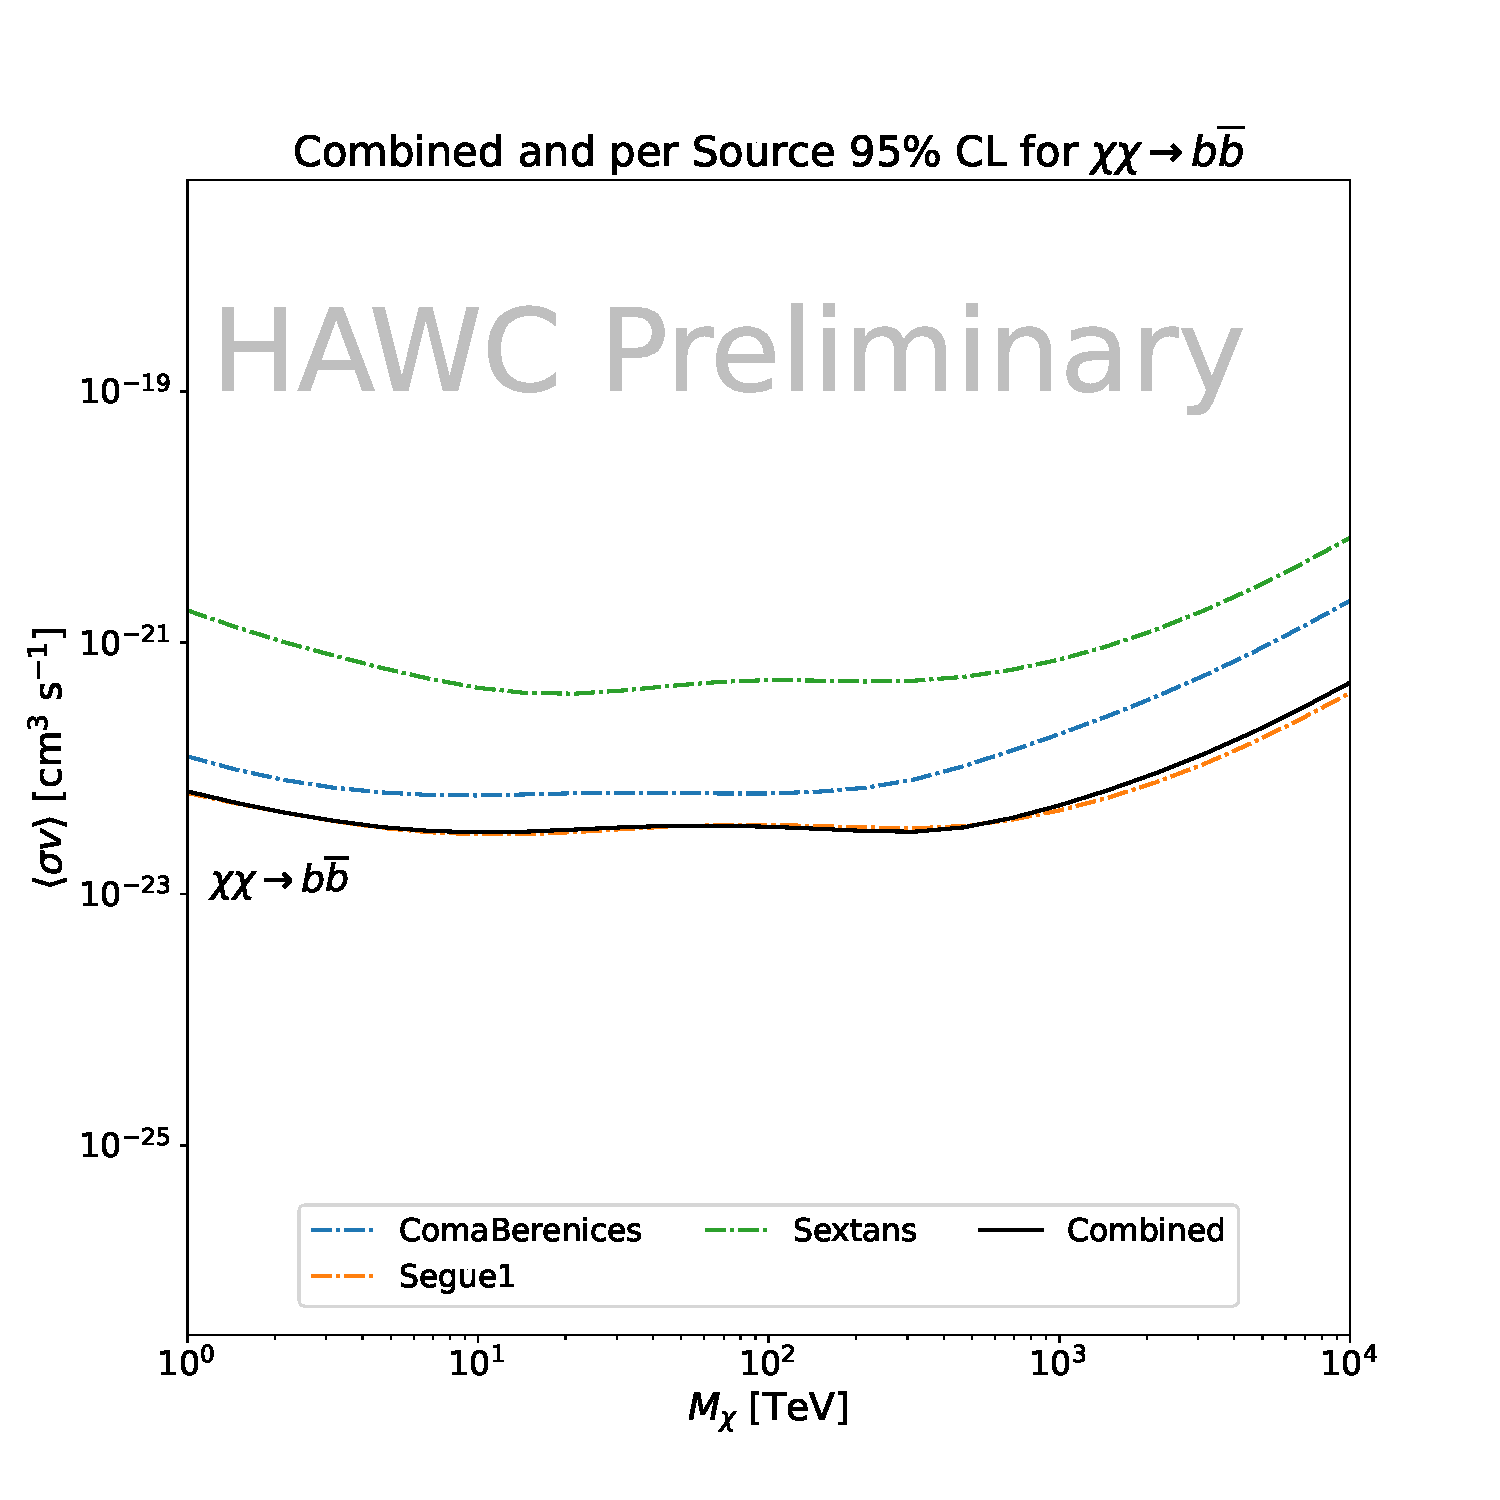
\includegraphics[scale=0.21]{figures/mtd_hawc_dm/results/Combined95_New_duck_bb_.pdf}
    }
    \caption{\todo{fill this out}}
\label{fig:mtd_limits_1of2}
\end{figure}

\begin{figure}[h]
\centering{
    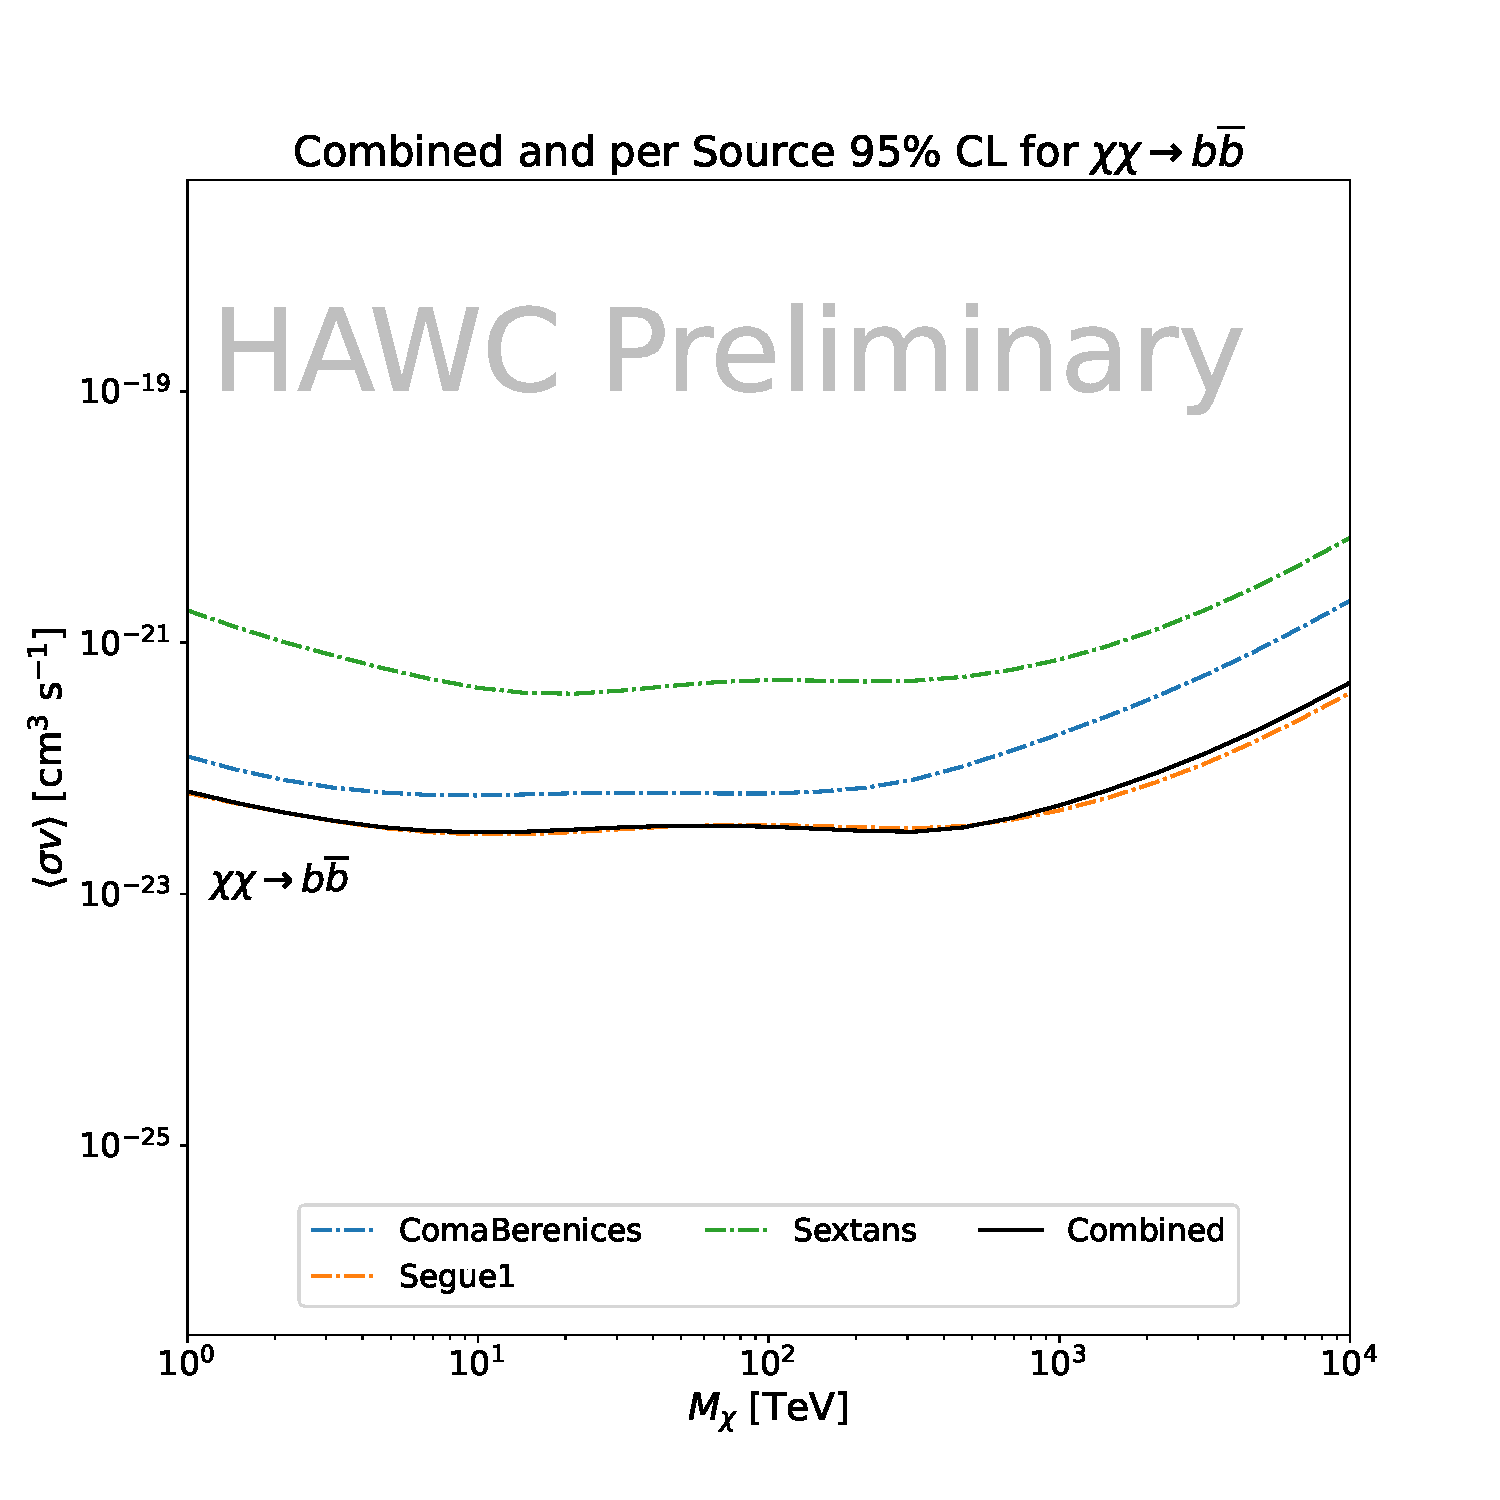
\includegraphics[scale=0.21]{figures/mtd_hawc_dm/results/Combined95_New_duck_bb_.pdf}
    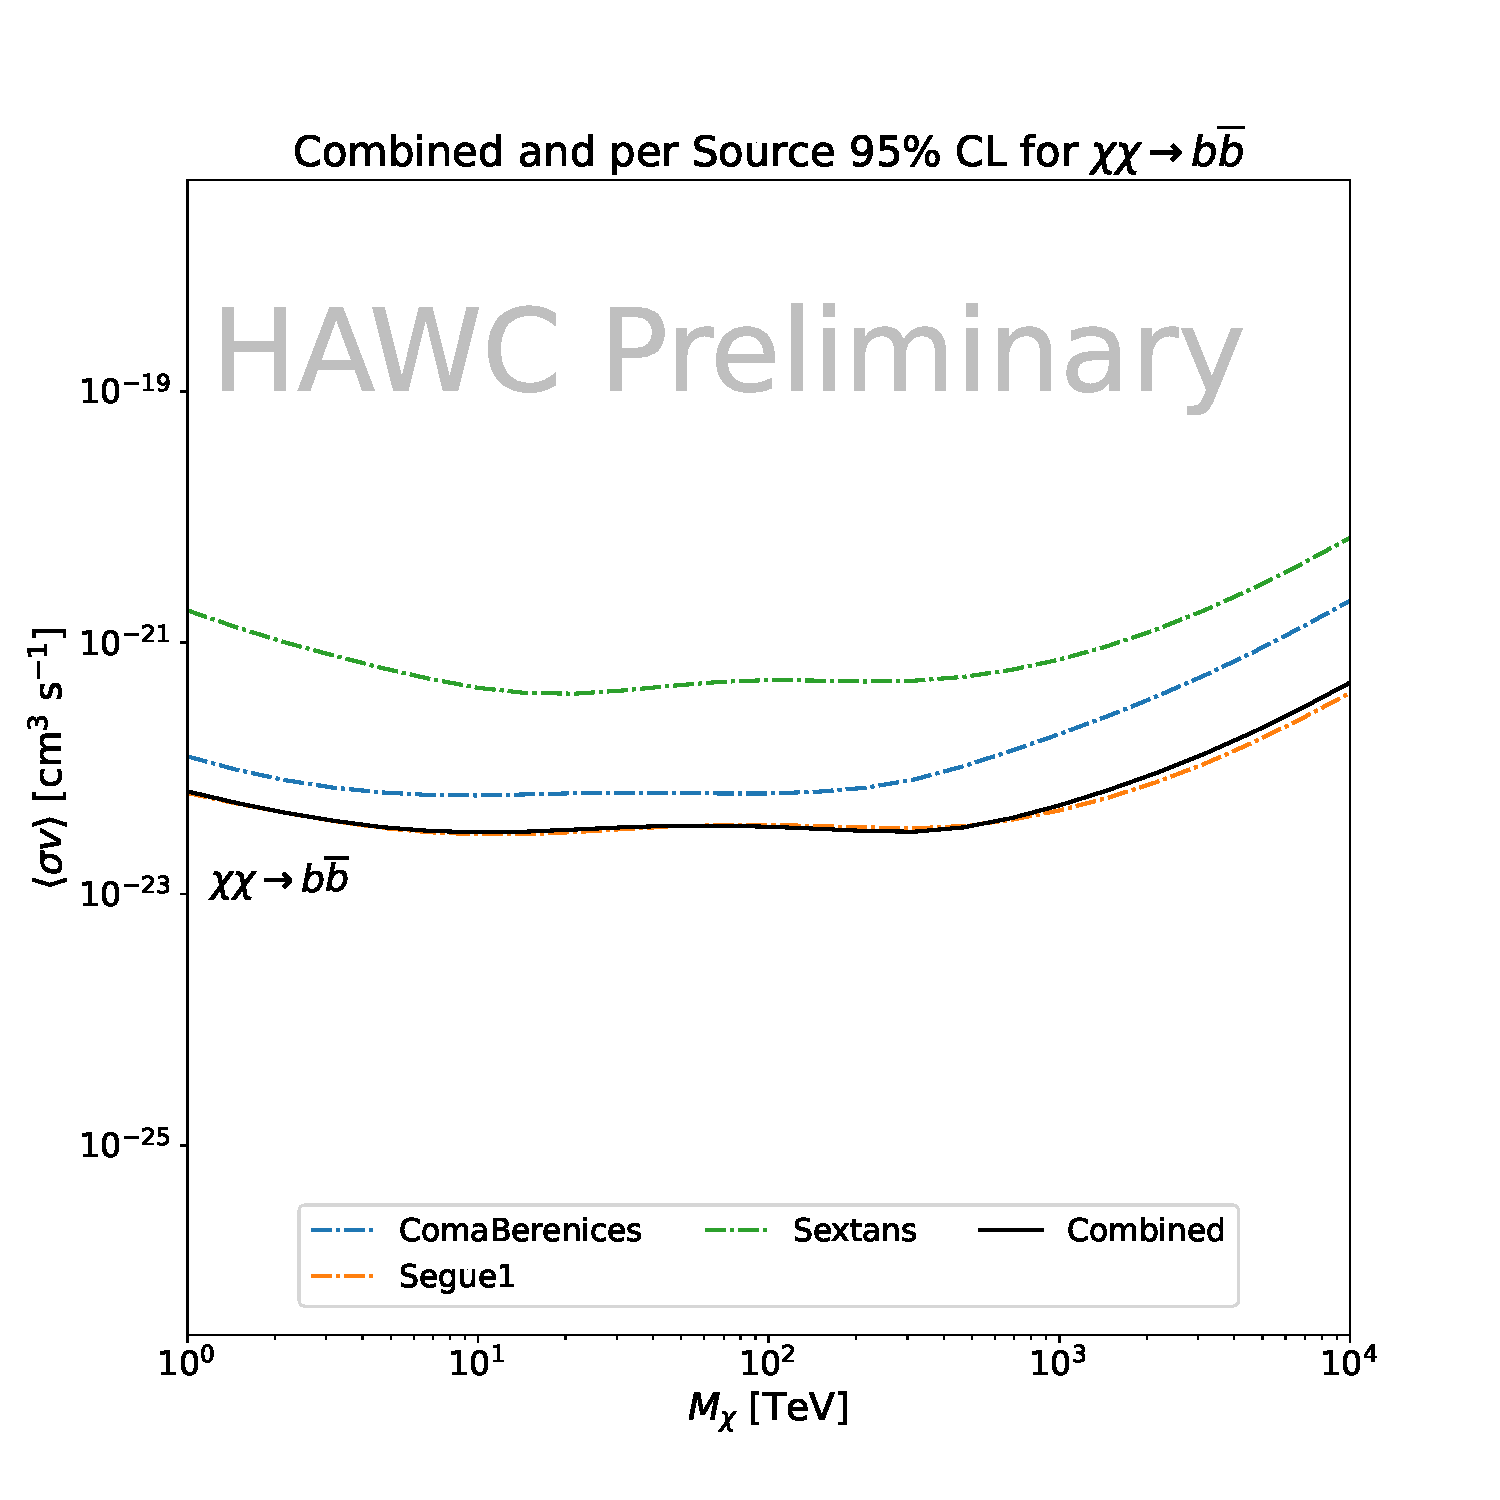
\includegraphics[scale=0.21]{figures/mtd_hawc_dm/results/Combined95_New_duck_bb_.pdf}
    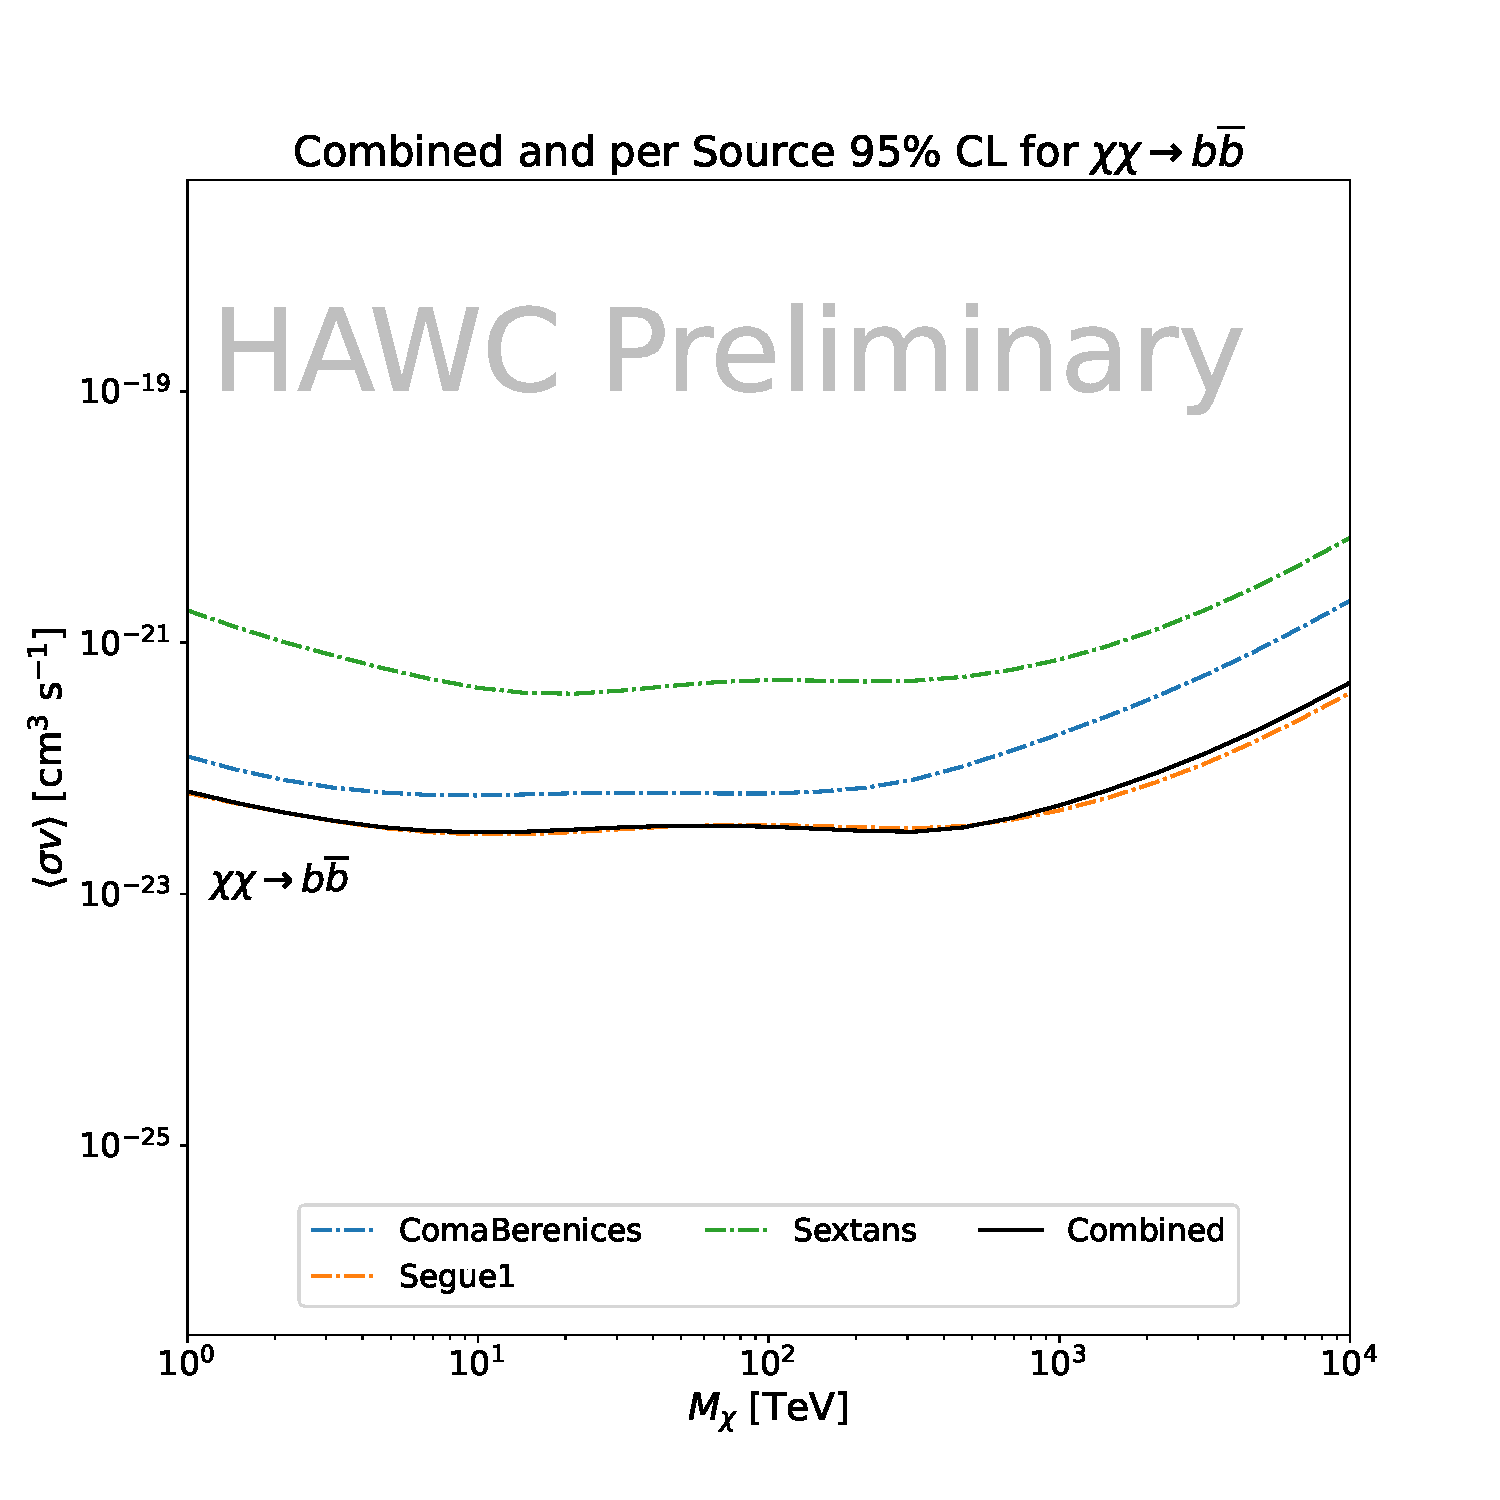
\includegraphics[scale=0.21]{figures/mtd_hawc_dm/results/Combined95_New_duck_bb_.pdf}
    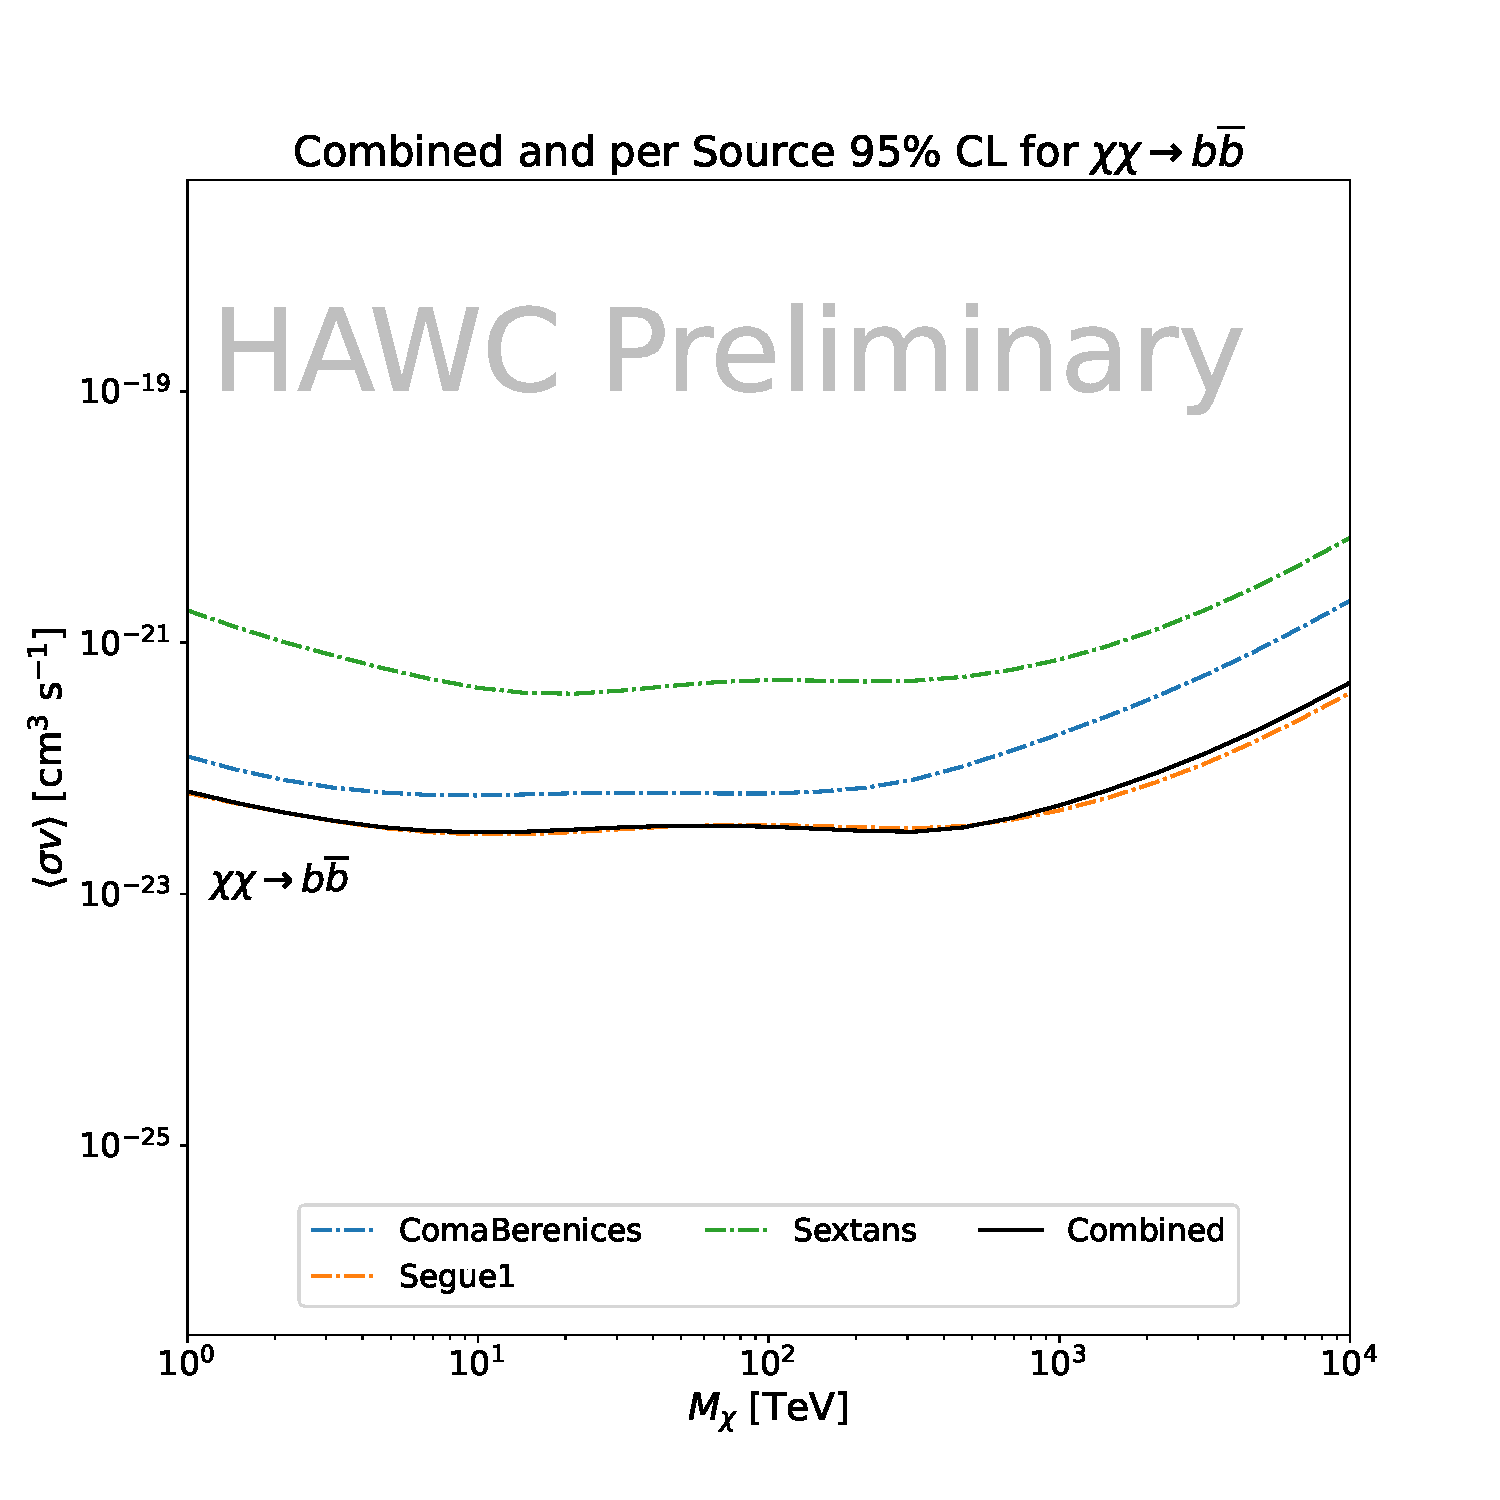
\includegraphics[scale=0.21]{figures/mtd_hawc_dm/results/Combined95_New_duck_bb_.pdf}
    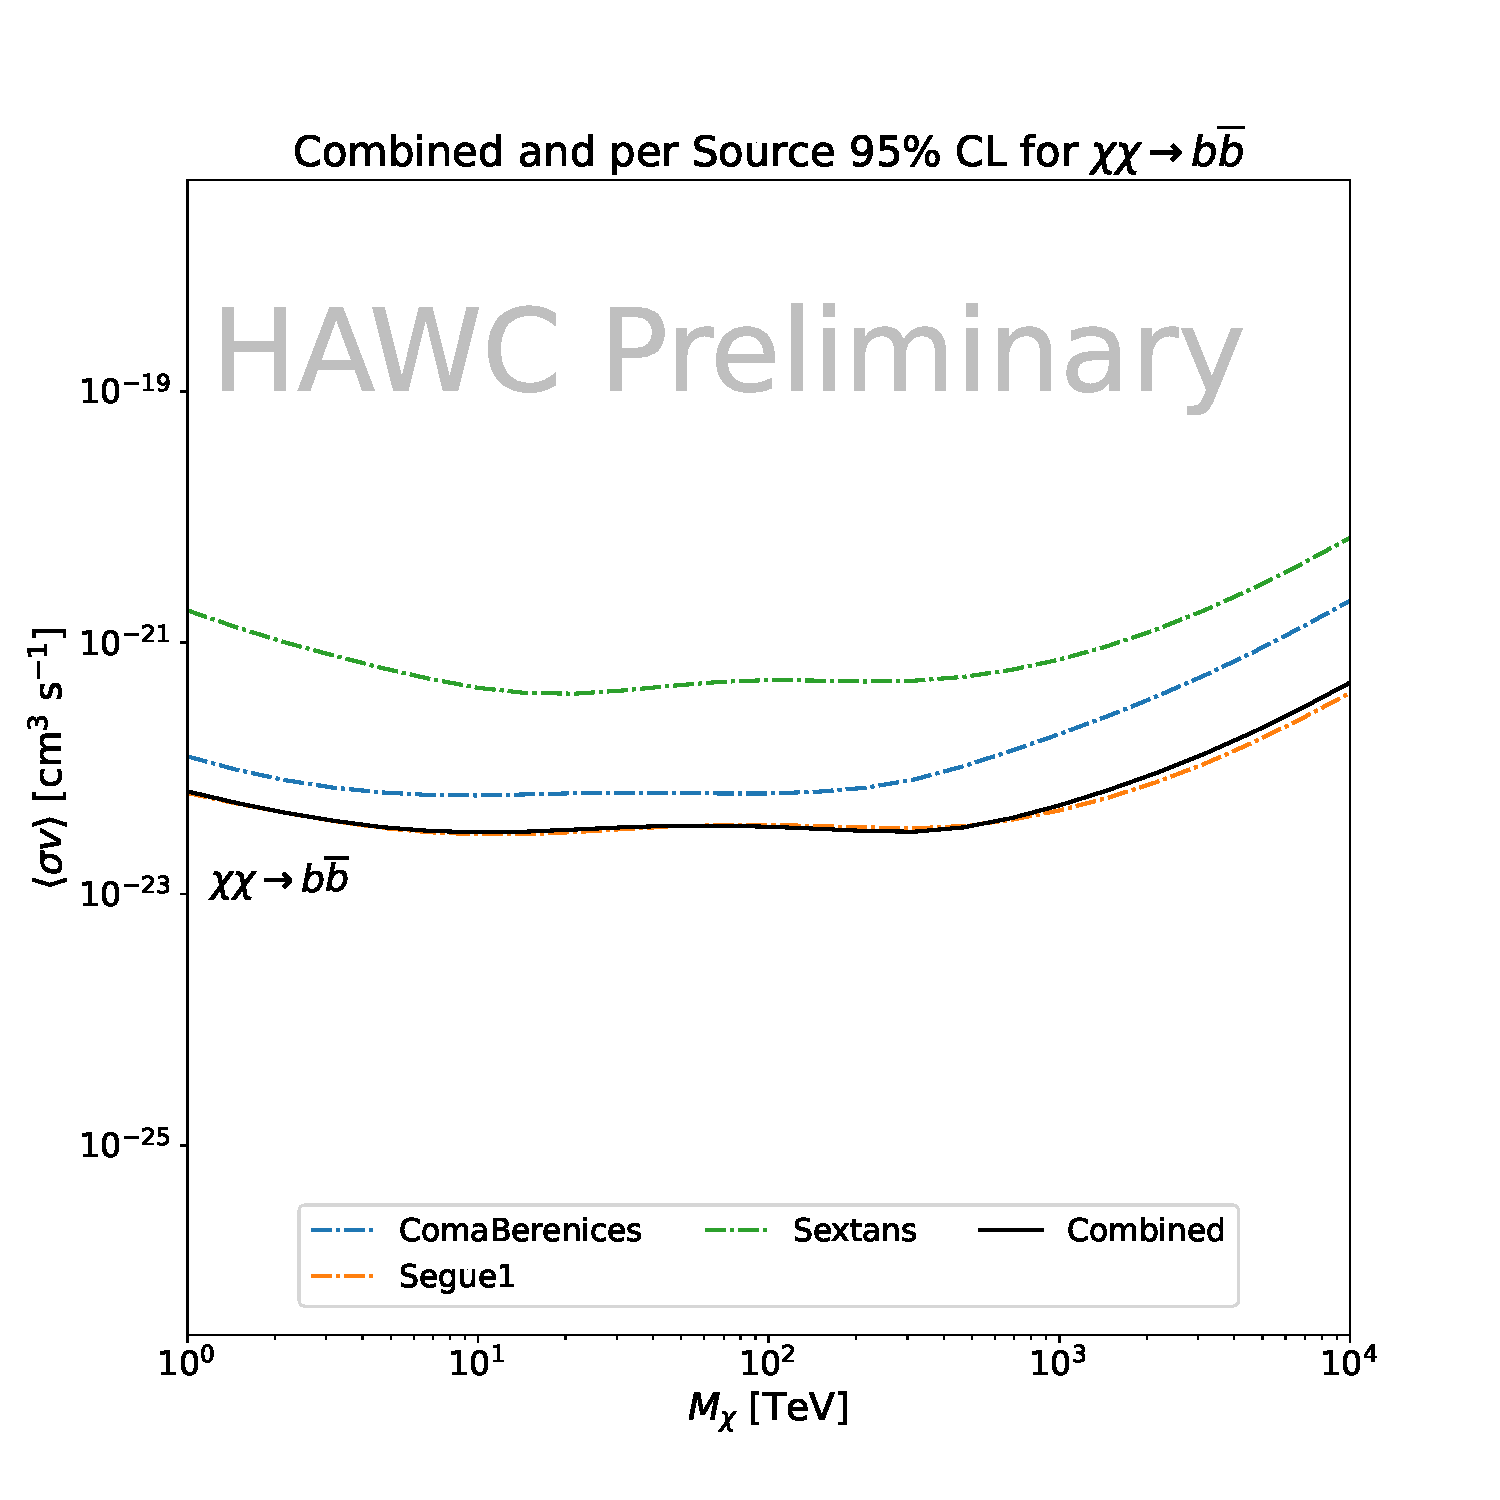
\includegraphics[scale=0.21]{figures/mtd_hawc_dm/results/Combined95_New_duck_bb_.pdf}
    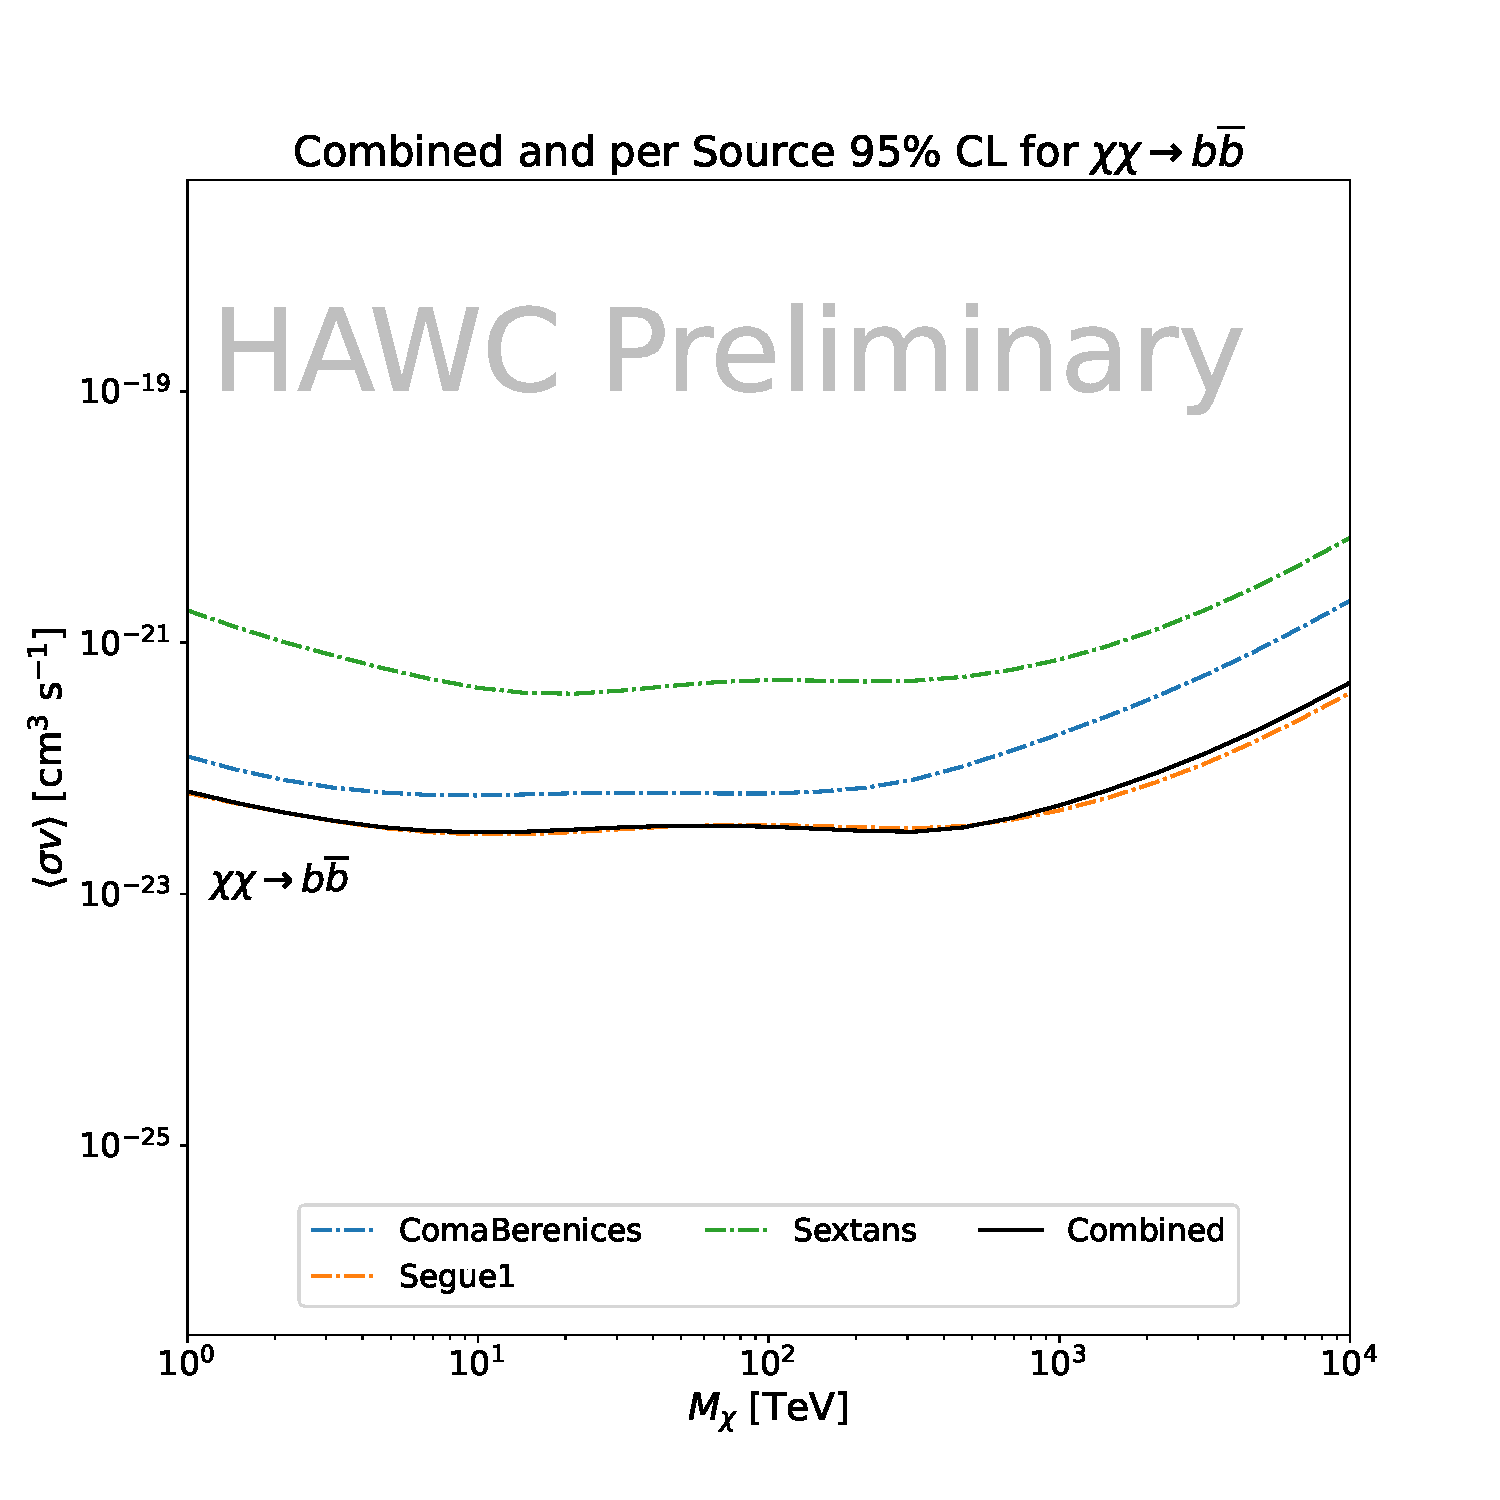
\includegraphics[scale=0.21]{figures/mtd_hawc_dm/results/Combined95_New_duck_bb_.pdf}
    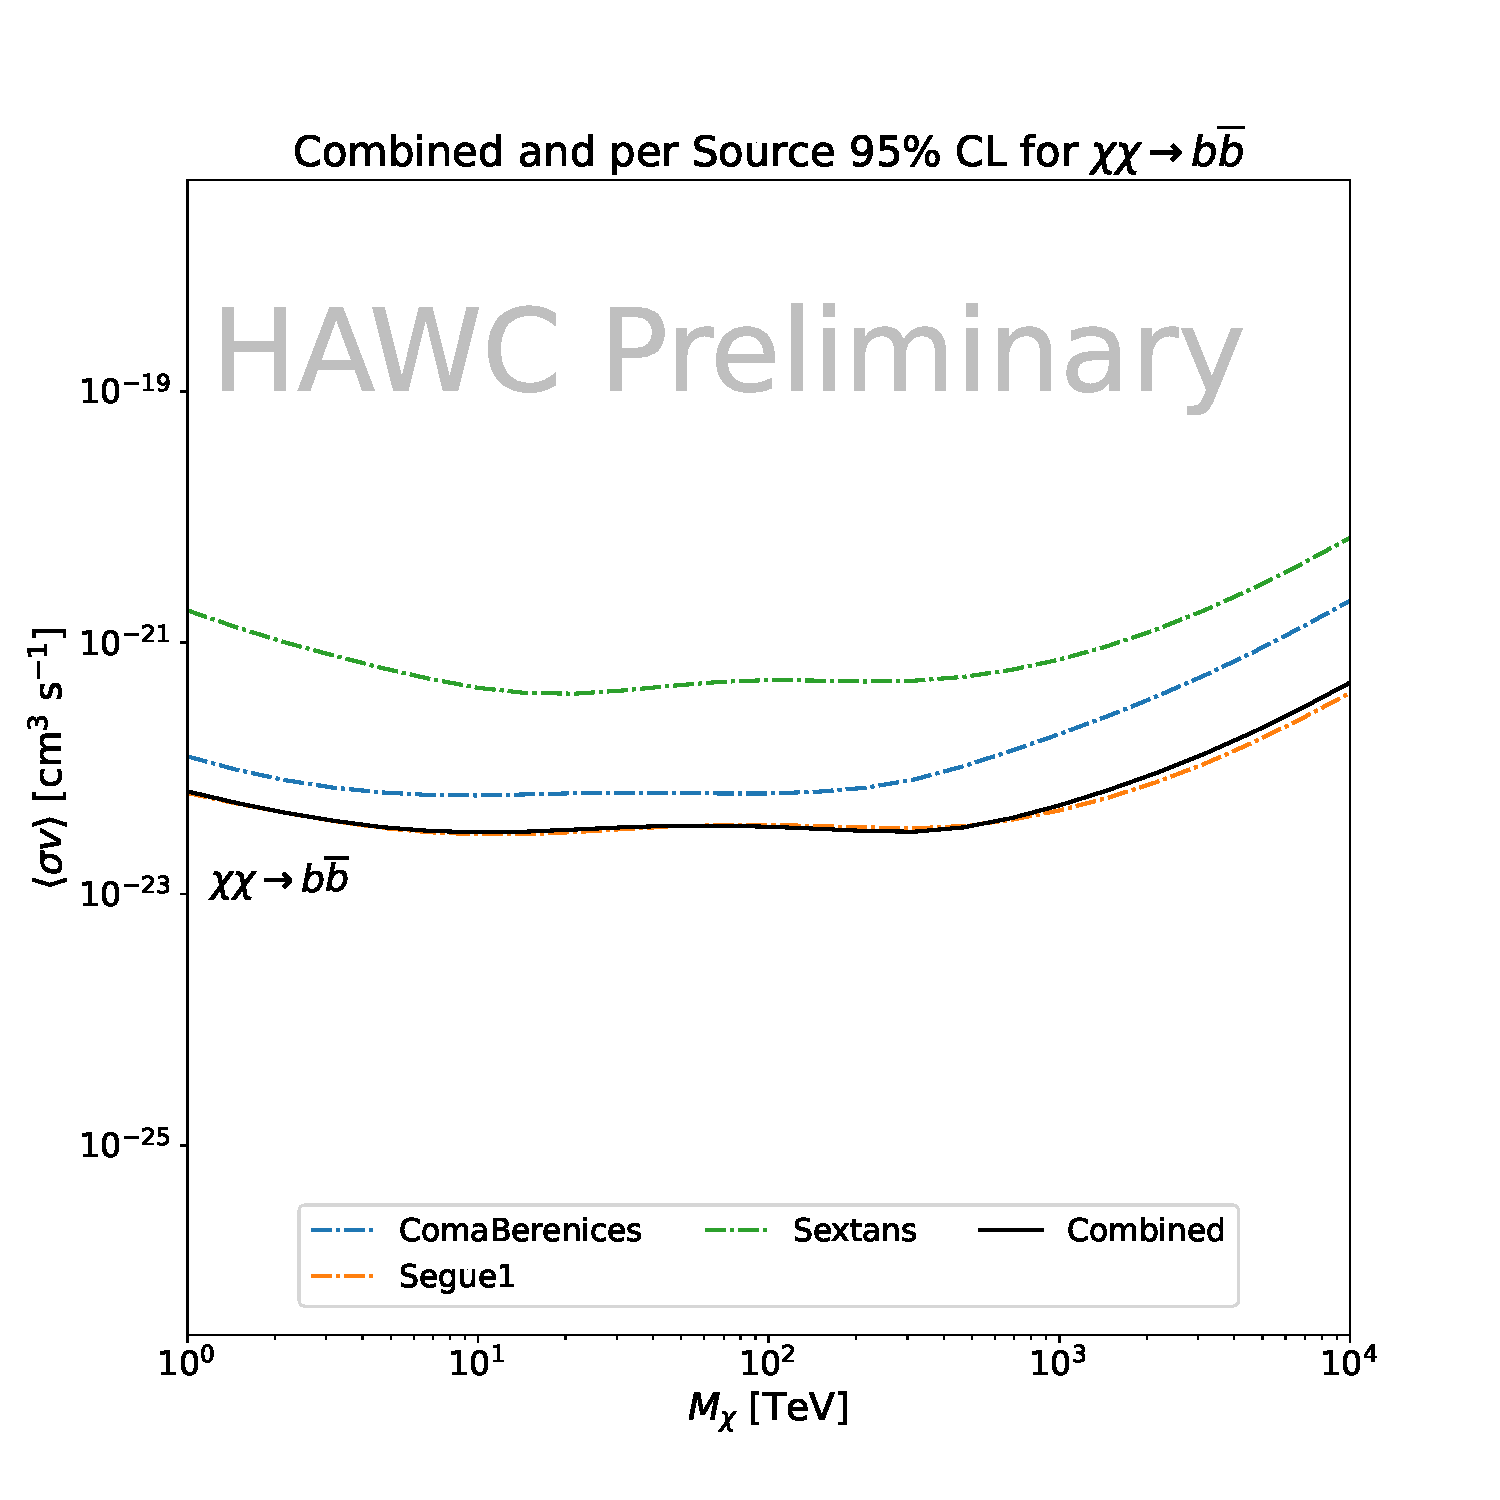
\includegraphics[scale=0.21]{figures/mtd_hawc_dm/results/Combined95_New_duck_bb_.pdf}
    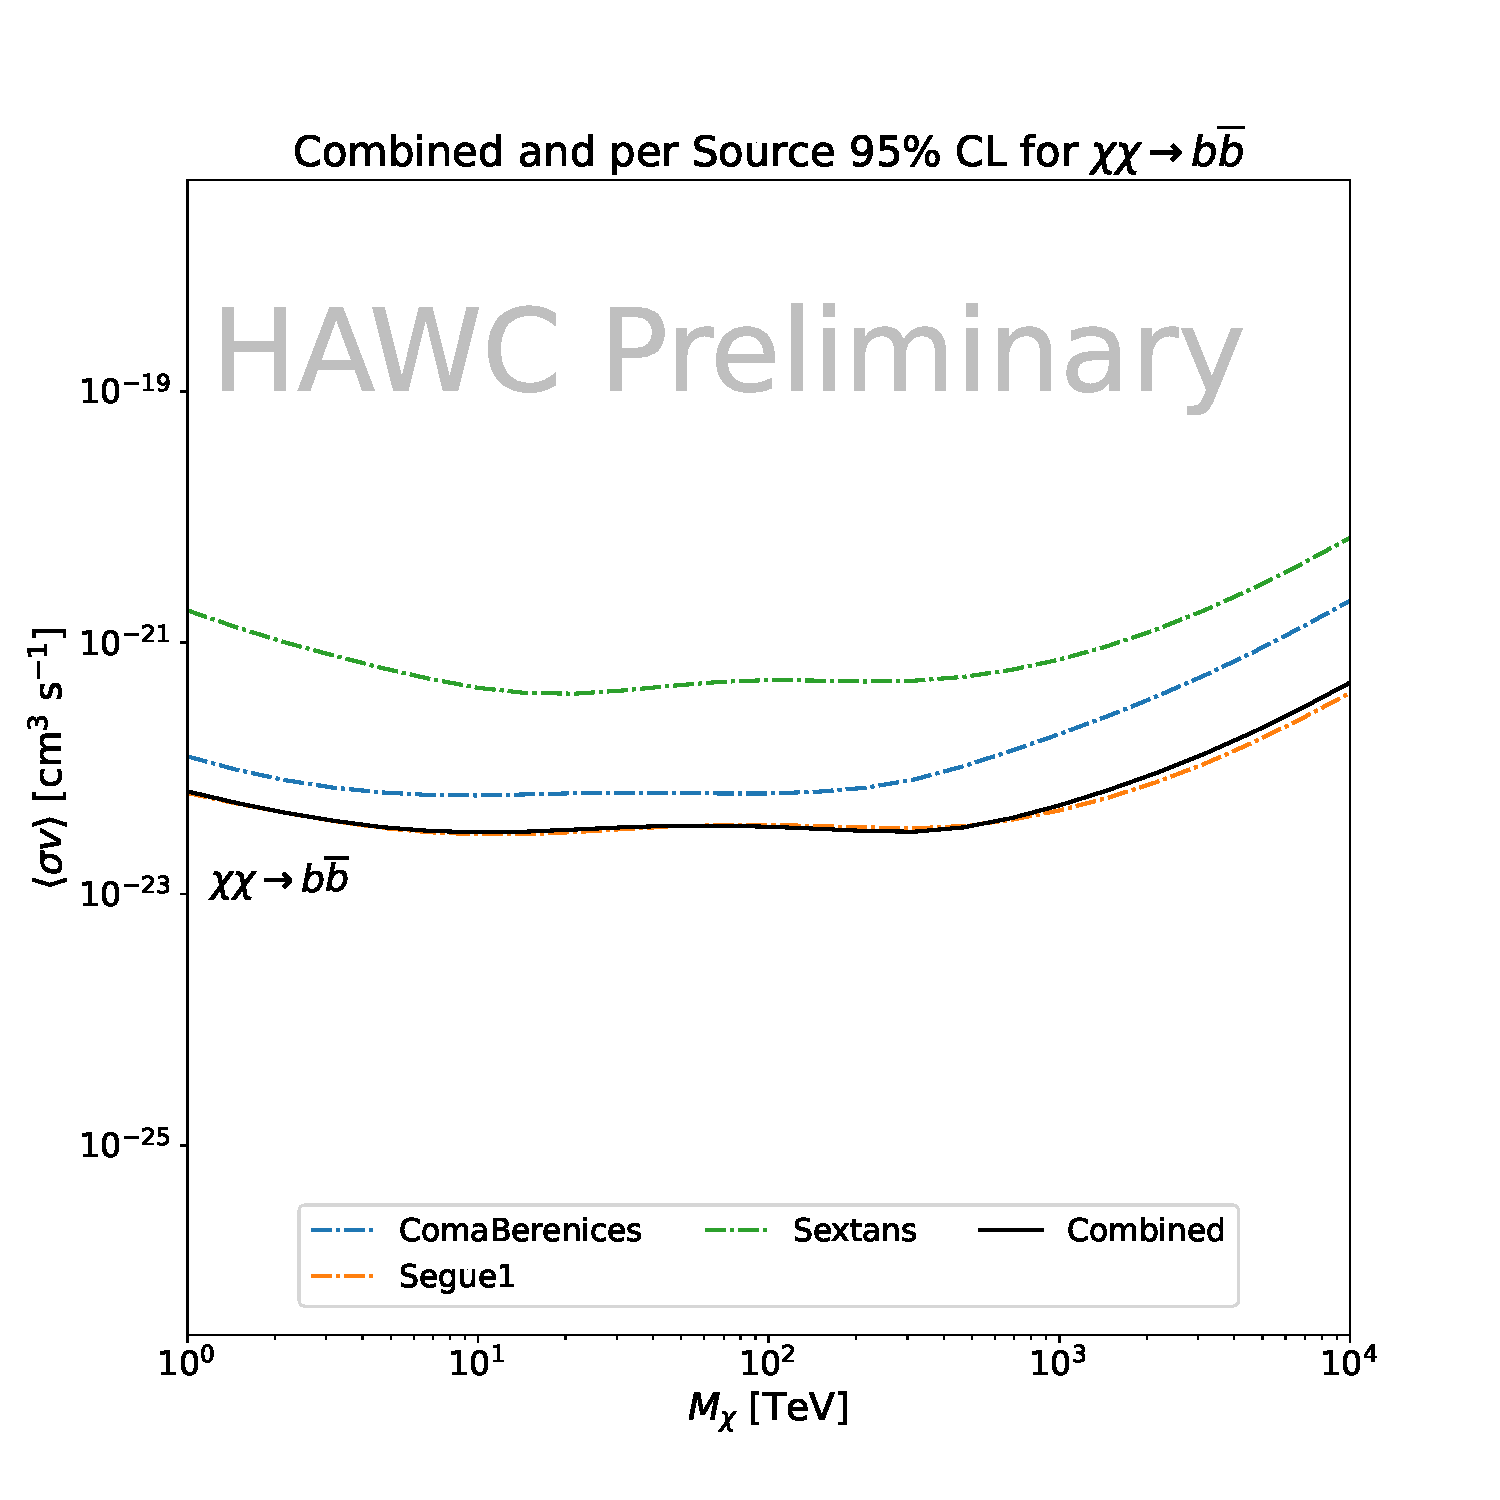
\includegraphics[scale=0.21]{figures/mtd_hawc_dm/results/Combined95_New_duck_bb_.pdf}
    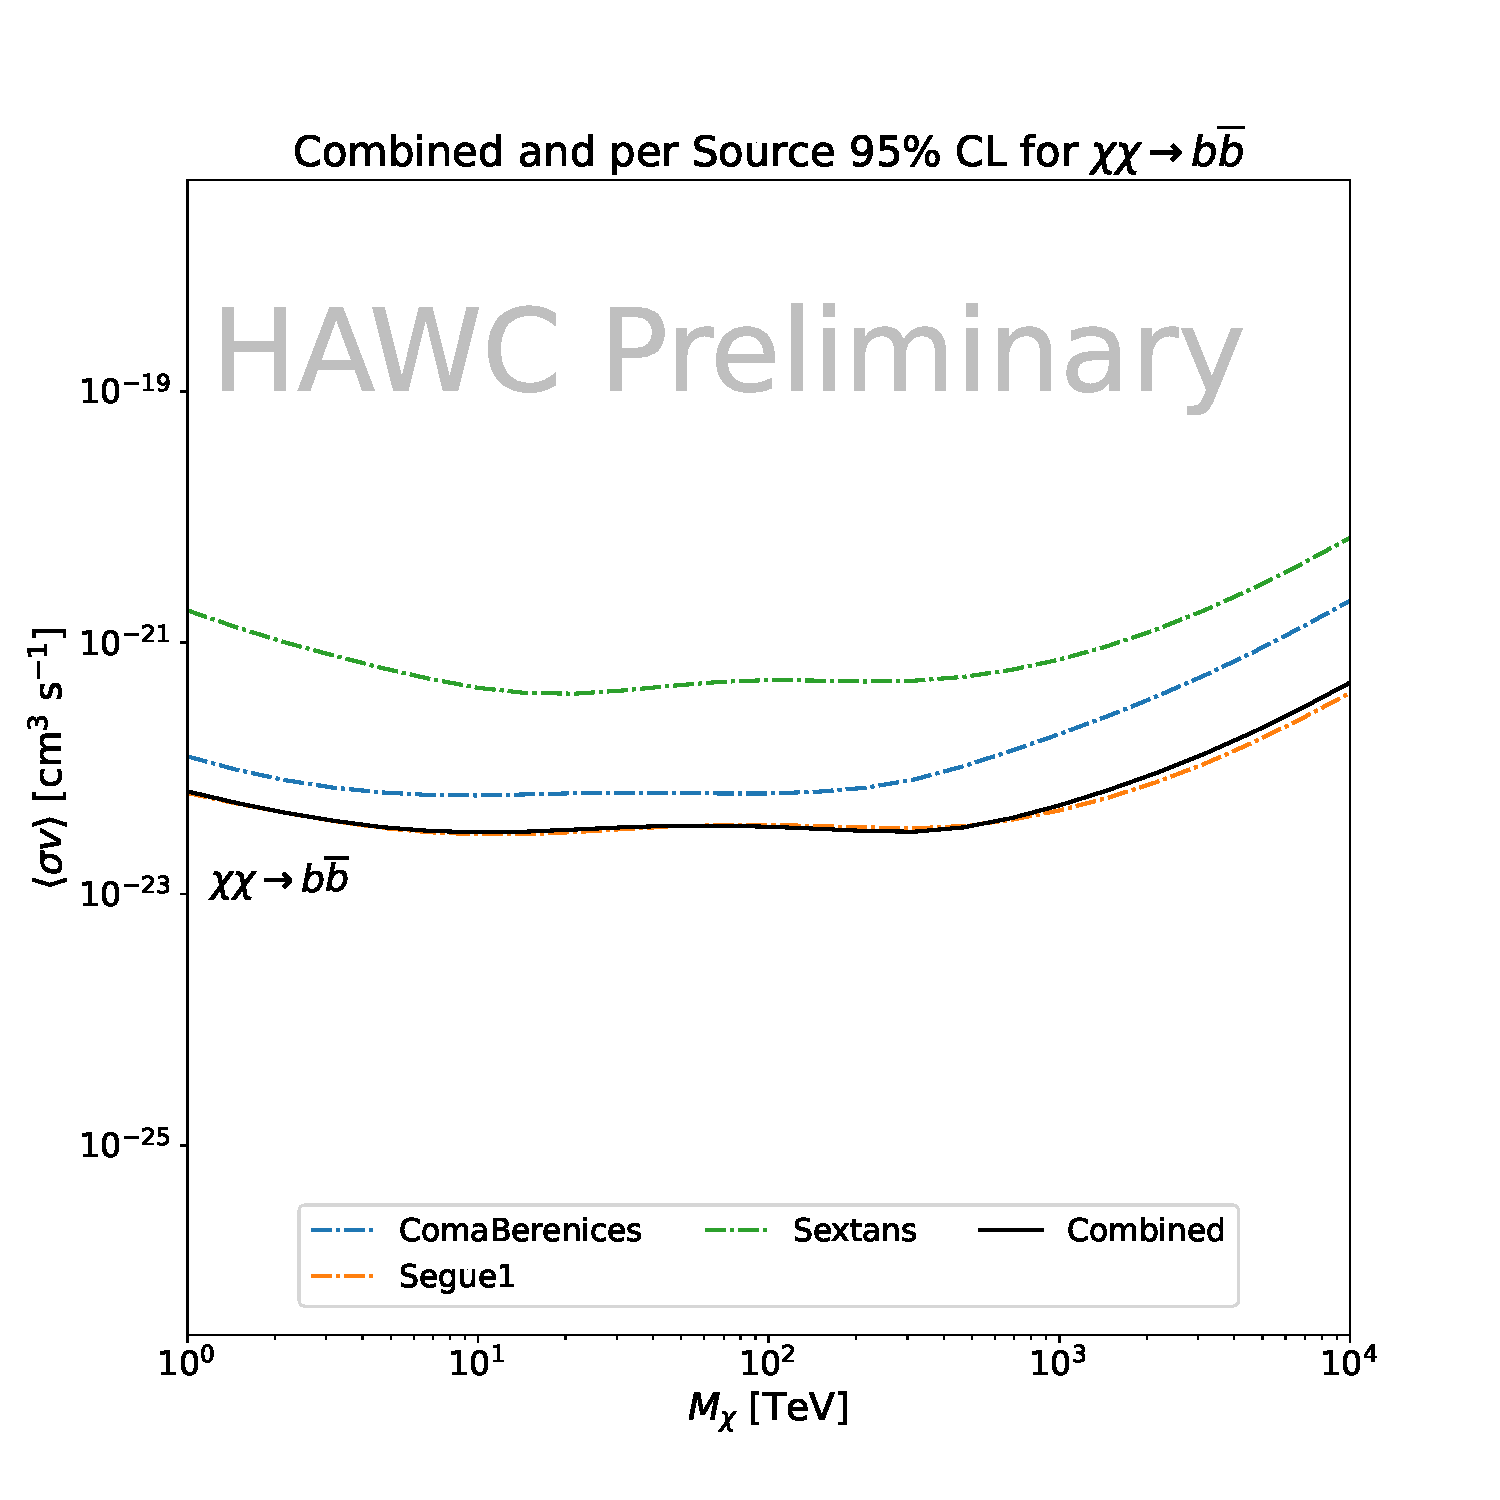
\includegraphics[scale=0.21]{figures/mtd_hawc_dm/results/Combined95_New_duck_bb_.pdf}
    }
    \caption{\todo{fill this out}}
\label{fig:mtd_limits_2of2}
\end{figure}

\tmpfig{TS of analysis of results. See if we can include Draco}
\tmpfig{TS of analysis of results. There will definitely be 2}

\tmpfig{Comparison of channels with GD combined results.}

\todo{talk about the results}

We were not able to generate background trials in time of writing this thesis.
These are not shown and are an immediate next step for this analysis before publication.

We did not see DM, but we did see some interesting excesses in the 10 Tev range at order $2\sigma$.
Draco was not included as the PDF of some of our analysis bins were wider than what is reasonable for a point source analysis.
Draco is at a high zenith for HAWC, so the effort required to include it was not justified by the benefits.


%%%%%%%%%%%%%%%%%%%%%%%%%%%%%%%%%%%%%%%%%%%%%%%%%%%%%%%%%%%%%
\section{Systematics}\label{sec:mtd_systemaics}
%%%%%%%%%%%%%%%%%%%%%%%%%%%%%%%%%%%%%%%%%%%%%%%%%%%%%%%%%%%%%

These are identical to what was performed earlier in Glory Duck, \cref{sec:hawc_systematic}.
We are also sensitive to the choice in spatial template, and this was explored in \cref{sec:gd_ext_limitvs_ptsrc} and \cref{sec:gd_gsVb}.

\LS also provided the uncertainty on their mean spatial models.
We perform a study on the $\pm 1\sigma$ spatial templates and show corresponding confidence limits in \todo{link to figure}

\tmpfig{show p1 and m1 limits around}
\tmpfig{there will be 2}

%%%%%%%%%%%%%%%%%%%%%%%%%%%%%%%%%%%%%%%%%%%%%%%%%%%%%%%%%%%%%
\section{Conclusion and Discussion}\label{sec:mtd_conclusion}
%%%%%%%%%%%%%%%%%%%%%%%%%%%%%%%%%%%%%%%%%%%%%%%%%%%%%%%%%%%%%

We want to include the remaining dSph and DM decay from the dSphs.
We saw an improvement of \todo{value} compared to Glory Duck which had many more dSphs.
\todo{copy some text from earlier section.}